\documentclass[11pt]{article}

\usepackage{amsmath}
\usepackage{amssymb}

\usepackage{graphicx}
\usepackage{float}
\usepackage{subcaption}
\usepackage{color}
\usepackage{tabularx, booktabs}

\newcommand{\od}[2]{\frac{d #1}{d #2}}
\newcommand{\pd}[2]{\frac{\partial #1}{\partial #2}}
\newcommand{\pdtwo}[2]{\frac{\partial ^2 #1}{\partial #2 ^2}}
\newcommand{\pdthree}[2]{\frac{\partial ^3 #1}{\partial #2 ^3}}

\begin{document}

\section{Introduction}

\subsection{Motivation}
The characterisation of low viscosity polymeric fluids is essential to many 
industrial applications. In particular extensional deformations of a fluid are 
encountered in coatings, lubrication and atomisation. The use of polymer 
additives is known to influence the stability and dynamics of jet break up, 
where the inhibition of `satellite' drops is desirable in inkjet printing for 
example.

The rheology of the fluid must therefore be ascertained in order to control 
such processes. These properties include the fluid relaxation time, the time 
taken for a fluid to return to its equilibrium state after a deformation, and 
the extensional viscosity. The transient uniaxial extensional viscosity is a 
function of the rate of stretching and is significantly different to the shear 
(dynamic) viscosity. For a Newtonian fluid \cite{fred1906coefficient} showed 
that the extensional viscosity is three times greater than the shear viscosity. 
For polymeric solutions this ratio can be orders of magnitude greater due to 
the microstructural contributions to the viscosity, where a coil to stretch 
transition of the polymers resists capillary thinning under an extensional 
deformation. The timescale of this transition is called the extensional 
relaxation time.

Currently, little is known about the extensional viscosity of dilute polymer 
solutions in comparison to the shear viscosity. This property is difficult to 
test experimentally for dilute polymer solutions due to the limited number of 
configurations in which a pure uniform extensional flow can be imposed in the 
laboratory and the effects of a pre-shear history on the polymer are difficult 
to control \citep{petrie2006extensional}.

To date filament stretching devices such as the Capillary Break up Extensional 
Rheometer (CaBER) have been shown to be able to probe relaxation in the range 
of 0.01 to 1 second \citep{bazilevsky1990liquid}. This device consists of two 
moving endplates where a liquid bridge is formed between the upper and lower 
liquid cusps. The thinning filament radius at the midpoint and the tensile 
forces are then measured. \cite{rodd2004capillary} showed that the 
characteristic time and length scales of the setup form a constraint on the 
operability of CaBER. This occurs when the Ohnesorge and Deborah numbers are 
both less than one. The Ohnesorge number is a dimensionless number which 
relates the viscous forces to the inertial and surface tension forces. The 
Deborah number characterises the elasticity and viscosity of a material. 
Therefore the operation of CABER is limited for weakly viscoelastic liquids 
such as dilute polymer solutions. These limitations results in elastic end 
plate instabilities where decohesion of the liquid bridge from the end plate 
occurs, or the fluid filament thinning much too rapidly for observations to be 
meaningful. 

Industrial applications require devices that can probe lower relaxation times 
that can be determined by CaBER. The Rayleigh Ohnesorge Jetting Extensional 
Rheometer (ROJER) employs an alternative approach to end plate stretching by 
following the dynamics of capillary driven jet break up, a new technique 
pioneered by \cite{keshavarz2015studying}. The significant advantage of this 
technique is the reduction in the characteristic length scale involved, from 
6mm for the plate diameter in CaBER to an initial nozzle diameter equal to 
200μm in ROJER. This allows ROJER to probe relaxation times down to the order 
of 60μs \citep{keshavarz2015studying}.

Utilising ROJER requires an understanding of the kinematics of the thinning jet 
filament. For a Newtonian fluid, this fundamentally consists of a force balance 
between the inertial, viscous and surface tension forces. For a polymeric 
fluid, additional elastic forces must be also considered. An overview of the 
theory underpinning capillary driven jet break up is given in the following 
section.

\subsection{History}
Leonardo da Vinci was the first to study the behaviour of liquid jets in the 
sixteenth century. He correctly identified that drop detachment was a force 
balance between gravitational forces and the surface tension of the fluid 
\citep{da1999codex}. However Da Vinci mistakenly assumed that this mechanism 
was also responsible for the dynamics of jet break up.

Much later, in the early nineteenth century, \cite{young1805essay} highlighted 
the stabilising and destabilising influence of surface tension during jet 
breakup and \cite{laplace1805traite} formulated a mathematical description of 
the mean curvature in order to describe the Laplace pressure. Fundamentally the 
surface tension force balances against the gravitational force during drop 
formation, but once a cylindrical shape of the fluid filament is reached the 
mean curvature destabilises the surface and detaches the drop.

\cite{savart1833memoire} significantly advanced experimental progress on the 
study of jet breakup shortly afterwards. He is credited with being the first to 
notice that the behaviour of jet break up is independent of the circumstances 
in which the jet is produced and developed a stroboscopic method where 
intermittent satellite drops were observed between two main drops. 

\cite{plateau1873statique} observed experimentally that surface tension works 
to reduce the surface area of the jet and that perturbations were unstable if 
the wavelength was greater than a critical value. \cite{strutt1878instability} 
subsequently introduced his method of linear stability analysis and discovered 
this critical wavelength is approximately nine times the initial jet radius, 
which is in good agreement with Savart's experiments conducted some fifty years 
earlier.

\cite{middleman1965stability} published a dispersion relation for a linearly 
viscoelastic jet based on the Oldroyd fluid model for a polymeric fluid. It was 
found that although viscoelasticity promotes instability at first, the 
unravelling of polymer chains at a critical strain rate resists the capillary 
thinning of the jet and therefore enhances stability.

\subsection{Aims and Objectives}
The aim of this report is to explore the capabilities of ROJER in 
characterising the intrinsic rheological properties of a fluid. This includes
\begin{itemize}
\item understanding the dynamics of extensional rheology using ROJER, from 
onset of the initial instability to capillary driven jet break up
\item the formulation of a Newtonian and a non-Newtonian one dimensional 
numerical simulation as a means to probe different aspects of jet behaviour 
with different dimensionless parameters, without the computational cost of 
solving the full Navier Stokes equations
\item the determination of an operating range for ROJER by testing different 
fluid materials, nozzle designs and dimensionless parameter spaces
\item the measurement of the extensional properties of various test fluids 
using ROJER and validating the results against theoretical predictions, one 
dimensional numerical simulations and computational fluid dynamics. 
\end{itemize}

\newpage

\section{The Stability Theory of Liquid Jets} \label{sec:stability}
A mathematical description of jet instability is detailed in this section. 
Firstly a linear inviscid jet is considered, then a description involving 
viscosity and then viscoelasticity will follow.

The Navier Stokes equation for an incompressible, Newtonian jet of density 
$\rho$, pressure $p$ and dynamic viscosity $\mu$ is given by
\begin{align}
\rho \left( \pd{\mathbf{u}}{t} + (\mathbf{u} \cdot \nabla) \mathbf{u} \right) 
= - \nabla p + \mu \nabla^2 \mathbf{u}
\label{eqn:navier}
\end{align}
where $\mathbf{u}$ is the fluid velocity field and $\nabla \cdot \mathbf{u} = 
0$. The capillary pressure at the jet surface is given by the Young-Laplace 
equation
\begin{align}
\Delta p &= \gamma \kappa \nonumber \\
&= \gamma \left(\frac{1}{R_1} + \frac{1}{R_2} \right)
\label{eqn:younglaplace}
\end{align}
where $R_1$ and $R_2$ are the principle radii of curvature, $\gamma$ is the 
surface tension and $\kappa$ is the mean curvature. Assuming the jet is 
axisymmetric along the $z$ axis with a free surface denoted  $R = R(z,t)$, then 
the mean curvature is
\begin{align}
\kappa &= \frac{1}{R_1} + \frac{1}{R_2} = \frac{1}{R(1+ R_z^2)^{1/2}} - 
\frac{R_{zz}}{(1 + R_z^2)^{3/2}}
\label{eqn:curvature}
\end{align}
where the subscript $z$ denotes a spatial derivative. Equations \ref{eqn:navier} 
and \ref{eqn:younglaplace} along with the incompressibility condition form the 
governing equations of the liquid jet.

To analyse the stability of a solution to these equations, a small perturbation 
is applied to an initial state. It is convenient to take the initial state to 
be $\mathbf{u}_0 = 0$, in other words along the reference frame moving at the 
jet velocity. The initial jet pressure is uniform and is equal to the Laplace 
pressure $p_0 = \gamma / R_0$ where $R_0$ is the initial jet radius.

\subsection{The Inviscid Jet}
\subsubsection{Rayleigh's Linear Stability Analysis}
In the case of an inviscid jet the viscosity $\mu$ is equal to zero. Therefore 
by the conservation of momentum and incompressibility there exists a condition 
on the pressure $p$  in a linear approximation where quadratic terms are 
ignored
\begin{align}
\nabla^2p = 0.
\label{eqn:laplace}
\end{align}
Axisymmetric perturbations are applied to the base state $\mathbf{u}_0 = 0$ and 
pressure $p = p_0$ which are of the form
\begin{align}
\mathbf{u}(r,z) = \mathbf{u}_0 + \tilde{\mathbf{u}}(r,z) \hspace{2cm} p(r,z) = 
p_0 + \tilde{p}(r,z)
\end{align}
where $r$ denotes the radial direction and $z$ the axial direction. Note that 
Equation \ref{eqn:laplace} is Laplace's equation and is solved analytically 
using the method of separation of variables. The result is that perturbed 
pressure must be of the form
\begin{align}
\tilde{p}(r,z) = F(r) \cos(kz)
\label{eqn:pressure_perturb}
\end{align}
where the function $F = F(r)$ satisfies the second order partial differential 
equation
\begin{align}
\pdtwo{F}{r} + \frac{1}{r} \pd{F}{r} -k^2 F = 0.
\label{eqn:pressure_diff}
\end{align}
The solution to Equation \ref{eqn:pressure_diff} is the modified Bessel 
function $F(r)=p'I_0(kr)$ with amplitude $p'$ and is bounded about $r=0$.

Turning to the jet surface it is required that the Laplace pressure is 
satisfied. A perturbation of the jet radius is defined as
\begin{align*}
R(z,t) &=  R_0 + \tilde{R} (z,t) \nonumber \\
& = R_0 + \delta_0 \exp(ikz + \alpha t),
\end{align*}
where $R_0$ is the initial radius of the jet. Substituting this into Equation 
\ref{eqn:laplace}, the pressure perturbation is given by
\begin{align*}
\tilde{p}(r=R_0,z) = -\frac{\gamma}{R_0^2} (1 - k^2 R_0^2) \, \delta_0 \exp(ikz 
+ \alpha t),
\end{align*}
Equating this pressure perturbation to Equation \ref{eqn:pressure_perturb} 
evaluated at $r=R_0$ relates amplitude $p'$ to the interface displacement 
$\delta_0$
\begin{align*}
p' = -\frac{\gamma}{R_0^2}(1-k^2 R_0^2) \frac{\delta_0 \exp (ikz + \alpha 
t)}{I_0(kR_0)}.
\end{align*}
Therefore the linearised expression for the pressure perturbation is given by
\begin{align}
\tilde{p}(r,z) = -\frac{\gamma}{R_0^2} (1 - k^2 R_0^2) \frac{I_0(kr)}{I_0 
(kR_0)} \, \delta_0 \exp(ikz + \alpha t).
\label{eqn:pressure_perturb_2}
\end{align}
The linearised kinematic condition at the jet surface states that
\begin{align}
\pd{\tilde{R}}{t} = \tilde{u}_r(r =R_0,z)
\label{eqn:kinematic}
\end{align}
and the linearised momentum equation states that
\begin{align}
\pd{\tilde{u}_r}{t} = - \frac{1}{\rho} \pd{\tilde{p}}{r}.
\label{eqn:r_momentum}
\end{align}
Combining Equations \ref{eqn:kinematic} and \ref{eqn:r_momentum} yields a time 
evolution equation for the jet surface
\begin{align}
\pdtwo{\tilde{R}}{t} = - \frac{1}{\rho} \pd{\tilde{p}}{r}(r = R_0, z).
\end{align}
Substituting the pressure perturbation from Equation \ref{eqn:pressure_perturb_2} 
into the evolution equation yields the dispersion relation
\begin{align}
\alpha^2 = \frac{\gamma k}{\rho R_0^2} (1 - k^2 R_0^2) \frac{I_1(kR_0)}{I_0(kR_0)}
\label{eqn:dispersion_rayleigh}
\end{align}
since $\od{I_0}{r} = I_1$, another Bessel function. This result was first 
obtained by \cite{strutt1878instability}.

The dispersion relation described by Equation \ref{eqn:dispersion_rayleigh} 
demonstrates the dependency of the growth rate $\alpha$ on the ratio of the 
surface tension $\gamma$ to the initial radius of the jet $R_0$. For the growth 
rate to have real and positive roots, the margin of stability is found to be $0 
< kR_0 <1$ which implies that $\lambda > 2 \pi R_0$. In other words all modes 
where the wavelength is greater than the initial jet perimeter are potentially 
unstable, as concluded by \cite{plateau1873statique}. By solving the dispersion 
relation \ref{eqn:dispersion_rayleigh} the maximum growth rate is given by 
\begin{align*}
\alpha^* = \frac{1}{3} \sqrt{\frac{\gamma}{\rho R_0^3}}
\end{align*}
corresponding to the wavenumber
\begin{align*}
k^*R_0 \approx 0.7.
\end{align*}
This is equivalent to a critical wavelength $\lambda^* = 9 R_0$. The 
characteristic time scale for the instability is chosen to be a balance between 
inertia and surface tension
\begin{align*}
t_R = \sqrt{\frac{\rho R_0^3}{\gamma}}.
\end{align*}

\subsubsection{The Long Wave Approximation}
Given that the critical mode (also known as the Rayleigh mode) occurs when the 
wavelength is approximately nine times the initial jet radius, then it is 
appropriate to seek a longwave approximation to the dispersion relation.

By assuming the wavelength is large then the wavenumber $kR_0$ is assumed to be 
much smaller than unity, therefore the modified Bessel functions which feature 
in Equation \ref{eqn:dispersion_rayleigh} reduce to their leading order terms, 
namely
\begin{align*}
I_0 = 1 \hspace{2cm} I_1 = \frac{kR_0}{2}.
\end{align*}
Therefore the long wavelength approximation of Equation 
\ref{eqn:dispersion_rayleigh} is
\begin{align}
\alpha^2 = \frac{\gamma k^2}{2 \rho R_0} (1 - k^2 R_0^2).
\label{eqn:dispersion_longwave}
\end{align}
This yields a non-dimensional maximum growth rate of 
\begin{align*}
\alpha^* t_R = \frac{1}{2 \sqrt{2}}.
\label{eqn:inviscid_max_growth}
\end{align*}
Figure \ref{fig:dispersion_compare} shows that there is a very good agreement 
between the long wavelength approximation (Equation \ref{eqn:dispersion_longwave}) 
and the exact dispersion relation (Equation \ref{eqn:dispersion_rayleigh}). The 
long wave approximation is less computationally expensive to solve than the 
full Navier Stokes equations and is found to be in excellent agreement 
according to Ambravaneswaran \cite{ambravaneswaran2002drop}.
\begin{figure}[h]
\begin{center}
	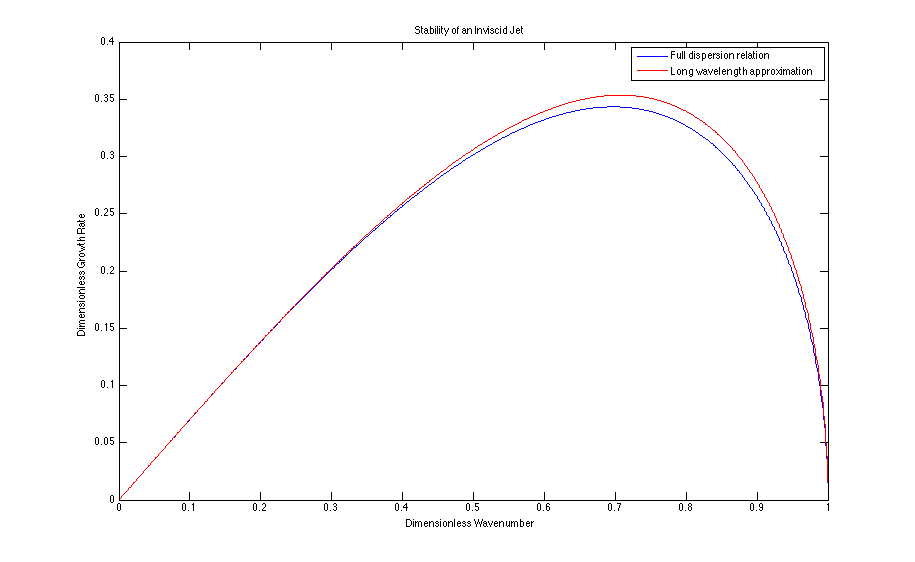
\includegraphics[width = 0.7\textwidth]{img/dispersion_comparison.png}
	\caption{The dimensionless wavenumber $kR_0$ against dimensionless growth 
rate $\alpha t_c$ for the exact dispersion relation \ref{eqn:dispersion_rayleigh} 
and the long wavelength approximation \ref{eqn:dispersion_longwave}.}
	\label{fig:dispersion_compare}
\end{center}
\end{figure} 

\subsubsection{The Critical Break Up Length of an Inviscid Jet} \label{sec:breakup_inviscid}
The critical break up length corresponds to the critical growth rate $\alpha^*$ 
given by Equation \ref{eqn:inviscid_max_growth}. The radius of this disturbance 
is expected to grow according to the Equation
\begin{align}
\tilde{R}(z,t) = \delta_0 \exp(ik^*z + \alpha^* t),
\end{align}
however the amplitude $\delta_0$ of this initial disturbance is unknown. The 
time taken $t^*$ for the perturbation to break up the jet can be found by 
assuming this corresponds to the time when $\tilde{R}(z,t) = R_0$. So the time 
taken for a perturbation at $z =0$ is
\begin{align*}
t^* = \frac{1}{\alpha^*} \ln \left( \frac{R_0}{\delta_0} \right) = \frac{C}{\alpha^*}
\end{align*}
where the constant $C$ replaces the unknown ratio between the amplitude of the 
initial disturbance and the initial radius of the jet. If the break up length 
is defined as $L^* = Ut^*$ then
\begin{align}
\frac{L^*}{D_0} = 3 C \, \mathrm{We}^{1/2}
\label{eqn:breakup_inviscid}
\end{align}
where the Weber number is defined as
\begin{align}
\mathrm{We} = \frac{\rho U^2 D_0}{\gamma}.
\end{align}
and non-dimensionalised by the initial jet diameter $D_0$. The Weber number is 
a useful dimensionless parameter in describing the ratio of fluid inertia to 
the surface tension. 

\subsection{The Viscous Jet}
\subsubsection{The Slender Jet Equations} \label{sec:slender}
The simplified analysis here involves the long wavelength description of the 
jet. Following \cite{eggers2008physics} the characteristic length scale $L$ and 
the time scale $T$ are chosen so that the balance of surface tension, inertia 
and viscous forces all enter the Navier Stokes equations at the leading order. 
That is,
\begin{align*}
L = \frac{\mu^2}{\gamma \rho} \hspace{2cm} T = \frac{\mu^3}{\gamma^2 \rho}.
\end{align*}
This reduces the $z$ component of the full incompressible Navier Stokes 
equation to
\begin{align*}
\rho \left( \pd{v}{t} + v \pd{v}{z} \right) = -\gamma \pd{\kappa}{z} + \frac{1}{R^2} 
\pd{}{z} \left(R^2 (\sigma_{zz} - \sigma_{rr}) \right).
\end{align*}
In the case where the fluid is Newtonian the stress tensor is defined as
\begin{align*}
\mathbf{\sigma} = \mu (\mathbf{K} + \mathbf{K}^T)
\end{align*}
where $K_{ij}$ is the velocity gradient tensor $K_{ij} = \pd{u_i}{x_j}$. The 
axial and radial stresses are therefore
\begin{align*}
\sigma_{zz} = 2\mu \pd{v}{z} \hspace{2cm} \sigma_{rr} = -\mu \pd{v}{z}
\end{align*}
so the Navier Stokes equation becomes
\begin{align*}
\rho \left( \pd{v}{t} + v \pd{v}{z} \right) = - \gamma \pd{\kappa}{z} + 3 \mu 
\frac{1}{R^2} \pd{}{z} \left(R^2 \pd{v}{z} \right).
\end{align*}
Additionally the kinematic equation reduces to a mass conservation law
\begin{align*}
\pd{R^2}{t} + \pd{}{z}(R^2 v) = 0.
\end{align*}
The full curvature term $\kappa$ in Equation \ref{eqn:curvature} is retained in 
order to preserve the accuracy beyond the limit where $|h_z| \ll 1$.

The slender jet equations can therefore be easily expressed in flux 
conservative form
\begin{align}
\pd{R^2}{t} + \pd{}{z} (R^2v) &= 0 \label{eqn:mass_con}
\end{align}
\begin{align}
\rho \left( \pd{}{t} (R^2v) + \pd{}{z} (R^2v^2) \right) &= \pd{}{z} \left(R^2 
\left( \gamma K + 3 \mu \pd{v}{z}\right) \right), \label{eqn:mom_con}
\end{align}
where
\begin{align*}
K \equiv \frac{1}{R(1+R_z^2)^{1/2}} + \frac{R_{zz}}{(1 + R_z^2)^{3/2}}.
\end{align*}

The slender jet equations form the basis for a one dimensional model of ROJER, 
which is verified in a team member report by \cite{hall2015report}.

\subsubsection{Linear Stability Analysis}
Consider small perturbations to the slender jet equations about the initial 
state for the free surface height and velocity
\begin{align*}
R(z,t) = R_0+ \tilde{R}(z,t) \hspace*{2cm} v = 0 + \tilde{v}(z,t)
\end{align*}
where the perturbations are of the form
\begin{align}
\tilde{R}(z,t) &= R' \exp(ikz + \alpha t) \nonumber \\
\tilde{v}(z,t) &= v' \exp(ikz + \alpha t).
\label{eqn:viscous_perturb}
\end{align}
in which $R'$ and $v'$ denote the amplitude of the perturbation, $k$ denotes 
the wavenumber and $\alpha$ denotes the growth rate. Substituting this into the 
mass conservation equation (Equation \ref{eqn:mass_con}) and linearising yields 
\begin{align}
2 \pd{\tilde{R}}{t} + R_0 \pd{\tilde{v}}{z} = 0.
\end{align}
Expanding this equation using the expressions in Equation \ref{eqn:viscous_perturb} 
gives a relation for the amplitude of the free surface height perturbation and 
the velocity perturbation
\begin{align}
R' = -\frac{1}{2} \frac{ik}{\alpha} v'.
\label{eqn:viscous_h}
\end{align}
Now substitute Equation \ref{eqn:viscous_h} into the momentum equation 
\ref{eqn:mom_con} and linearise to get
\begin{align*}
\rho R_0^2 \pd{\tilde{v}}{t} = \gamma \left( R_0^2 \pdthree{\tilde{R}}{z} + 
\pd{\tilde{R}}{z} \right) + 3 \mu R_0^2 \pdtwo{\tilde{v}}{z}.
\end{align*}
Expanding this equation using the expressions in Equation \ref{eqn:viscous_perturb} 
yields
\begin{align*}
\left(\alpha + \frac{3 \mu k^2}{\rho} \right) v' = \frac{\gamma}{\rho R_0}(1 - 
k^2 R_0^2) i k h'.
\end{align*}
Eliminating $h'$ using the relation in Equation \ref{eqn:viscous_h} gives the 
dispersion relation for viscous jets
\begin{align}
\alpha^2 + \frac{3 \mu k^2}{\rho}\alpha - \frac{\gamma k^2}{2 \rho R_0}(1 - 
k^2R_0^2) = 0.
\label{eqn:dispersion_viscous}
\end{align}
As expected, the long wave description of the dispersion relation for an 
inviscid jet is  (Equation \ref{eqn:dispersion_longwave}) is recovered when 
$\mu =0$. The dispersion relation also reveals that the maximum growth rate is 
\begin{align}
\alpha^*t_R = \frac{1}{2 \sqrt{2} + 6 \, Oh}
\label{eqn:visc_max_growth}
\end{align}
where the Ohnesorge number is defined as
\begin{align}
Oh = \frac{\mu}{\sqrt{\rho \gamma R_0}}.
\end{align}
The corresponding critical wavenumber is
\begin{align}
k^*R_0 = \frac{1}{\sqrt{1+ 3\sqrt{2} \, Oh}}.
\end{align}
Figure \ref{fig:dispersion_viscous} shows the deformation of the dispersion 
curve with increasing Ohnesorge number. Viscous forces dampen the growth rate 
of the perturbation as expected and the value of most unstable wavelength 
increases for more viscous jets.
\begin{figure}[ht]
\begin{center}
	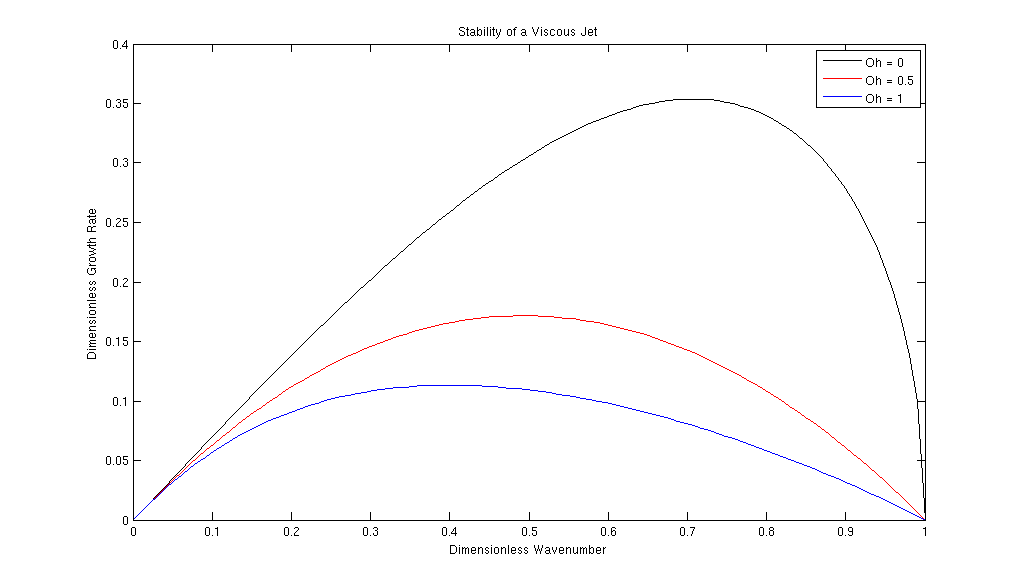
\includegraphics[width = 0.7\textwidth]{img/dispersion_comparison_viscous.png}
	\caption{The dimensionless wavenumber $kR_0$ against dimensionless growth 
rate $\alpha t_R$ for varying Ohnesorge numbers in the long wavelength 
approximation. Increasing fluid viscosity reduces the value of the growth rate 
and the critical wavelength for the most amplified mode increases.}
	\label{fig:dispersion_viscous}
\end{center}
\end{figure}

\subsubsection{The Critical Break Up Length of Viscous Jets} \label{sec:breakup_length}
Following a similar derivation outlined in Section \ref{sec:breakup_inviscid}, 
the critical break up length of a viscous jet is given by
\begin{align}
\frac{L^*}{D_0} = C \, \mathrm{We}^{1/2}(2 \sqrt{2} + 6 \, Oh)
\label{eqn:breakup_viscous}
\end{align}
where the Ohnesorge number is non-dimensionalised using $D_0$ also. From 
Equation \ref{eqn:breakup_viscous} it can be seen the break up length of the 
jet increases with viscosity as the length of the most unstable wavelength 
increases, which is also reflected in Figure \ref{fig:dispersion_viscous}.

\subsection{The Viscoelastic Jet}
This section incorporates the viscoelastic effects of the Oldroyd B model 
\citep{oldroyd1950formulation} into the slender jet equations derived in 
Section \ref{sec:slender}. This constitutive model is one of the simplest 
models for polymeric fluids in which polymers are described by Hookean bead 
spring dumbbells.

%\subsubsection{The Storage and Loss Moduli}
%The axial and radial stresses in Equation \ref{eqn:mom_con} are determined by 
their relationship with the strain rate \cite{goldin1969breakup}, most 
generally described by
%\begin{align}
%\sigma_{ij} = \int^t_{-\infty} G(t - t')E_{ij}(t') dt'
%\end{align}
%where $G(t)$ is the elastic modulus and $E_{ij}$ is the strain rate tensor.
%
%The elastic modulus $G(t)$ is obtained experimentally via an oscillatory shear 
experiment, usually a Couette device. A homogeneous shear is imposed on the 
flow  of the form
%\begin{align*}
%\gamma(t) = \gamma_0 \sin (\omega t)
%\end{align*}
%where $\gamma_0$ is the amplitude of the shear and $\omega$ is the frequency. 
The shear rate is 
%\begin{align*}
%\dot{\gamma}(t) = \gamma_0 \omega \cos (\omega t).
%\end{align*}
%and therefore the stress in the flow is
%\begin{align*}
%\sigma(t) = \int^t_{-\infty} G(t-t') \gamma_0 \omega \cos (\omega t') \, ds.
%\end{align*}
%A variable substitution $s = t-t'$ yields
%\begin{align*}
%\sigma(t) &= \gamma_0 \omega \int^t_{-\infty} G(s) \cos(\omega(t-s)) \, ds \\
%&= \gamma_0 \omega \int^t_{-\infty} G(s) \Re\left[\exp (i \omega (t-s)\right] 
\, ds \\
%& = \gamma_0 \omega \Re \left[ \exp(i \omega t) \int^\infty_0 G(s) \exp(-i 
\omega s) \, ds \right].
%\end{align*}
%By convention, the complex shear modulus $G*$ is defined as
%\begin{align*}
%G^* (s) = i \omega \int^\infty_0 G(s) \exp (-i \omega s) \, ds
%\end{align*}
%with real and imaginary parts
%\begin{align*}
%G^* = G^* + i G''
%\end{align*}
%where $G'$ is called the storage modulus and $G''$ is the loss modulus. 
Therefore the expression for the stress becomes
%\begin{align}
%\sigma (t) &= \gamma_0 \Re \left[ \exp (i \omega t) (-i G^*(t)) \right] 
\nonumber \\
%&= \gamma_0 \left[ G'(t) \sin (\omega t) + G''(t) \cos (\omega t) \right] 
\nonumber \\
%&= \gamma (t) G'(t) + \frac{\dot{\gamma}(t)}{\omega} G''(t).
%\end{align}
%It can be seen that storage modulus is in phase with the shear and describes 
the fluids ability to store elastic energy. The loss modulus is in phase with 
the shear rate and describes the dissipation of energy, in other words the 
viscosity. Therefore
%\begin{align}
%\mu'= \frac{G''}{\omega}
%\end{align}
%is defined as the effective viscosity of the polymeric fluid.
%
%\subsubsection{The Oldroyd B Model} \label{sec:oldroyd}
%For an Oldroyd B fluid the storage and loss moduli are defined as
%\begin{align*}
%G' = \frac{G \omega^2 \tau^2}{1 + \omega^2 \tau^2} \hspace{2cm} G'' = \mu_s 
\omega + \frac{G \omega \tau}{1+\omega^2 \tau^2}.
%\end{align*}
%Therefore the viscosity 

A simple Oldroyd B approximation to the viscosity of a viscoelastic fluid is a 
summation of the solvent viscosity and the polymer contribution. 
\begin{align}
\mu(\alpha) = \mu_s + \frac{G \tau}{1 + \alpha \tau}
\end{align}
where $G$ is the elastic modulus and $\tau$  is the relaxation time. Therefore 
the slender jet approximation of the momentum equation becomes
\begin{align*}
\rho \left( \pd{}{t} (h^2v) + \pd{}{z} (h^2v^2) \right) = \pd{}{z} \left(h^2 
\left( \gamma K + 3 \mu(\alpha) \pd{v}{z}\right) \right).
\end{align*}
Therefore the dispersion relation is
\begin{align}
\alpha^2 + \frac{3 \mu(\alpha) k^2}{\rho}\alpha - \frac{\gamma k^2}{2 \rho 
R_0}(1 - k^2R_0^2) = 0
\label{eqn:dispersion_viscoelastic}
\end{align}
which is similar in form to the viscous Newtonian case (Equation 
\ref{eqn:dispersion_longwave}). The maximum growth rate is
\begin{align*}
\alpha^* t_R = \frac{1}{2 \sqrt{2} + 6 Oh_{\mu^*}}
\end{align*}
where
\begin{align*}
Oh_{\mu^*} = \frac{\mu(\alpha^*)}{\sqrt{\rho \gamma R_0}}.
\end{align*}
This model ensures that the viscosity is a monotonically decreasing function of 
the growth rate with the solvent viscosity $\mu_s$ being the lower limit. 

\subsection{The Dynamics of Jet Break Up}
In approach to the break up of the jet the radius $R$ approaches zero, which 
creates a singularity in the curvature term $K$ in the slender jet equations 
(see Equations \ref{eqn:mass_con} and \ref{eqn:mom_con}). This means that break 
up behaviour is independent of the initial or boundary conditions since the 
scales involved are significantly different. It is therefore appropriate to 
look for a self similar solution by choosing a suitable scale transformation. 
The details of the asymptotic scaling laws are not within the scope of this 
report but are derived by \cite{eggers2005drop}.

\subsubsection{The Universal Eggers Regime}
A stable similarity solution predicts that a Newtonian jet will have a minimum 
radius of
\begin{align}
R_{min} = 0.0304 \left( \frac{\gamma}{\mu} \right) \left(t_b - t \right)
\label{eqn:eggers}
\end{align}
where $t_b$ indicates the time to break up. Since this result is independent of 
the initial or boundary conditions, Equation \ref{eqn:eggers} is universal. 
However there exists a critical Ohnesorge number which forms a boundary where 
the dynamics are initially governed by an inertial or viscous regime. Either 
regime will eventually transition to the universal Eggers regime in the last 
stages of pinching. The radius at which this final transition occurs is often 
beyond the scale of observation in experiment, but is verified numerically 
using the one dimensional slender jet equations \citep{hall2015report}.

\subsubsection{The Inertial Regime}
The similarity solution for an inertially dominated Newtonian jet was derived 
by \cite{day1998self} from the full inviscid Navier Stokes equations, as the 
profile of the jet overturns if the slender jet equations are evaluated. The 
solution for $Oh \ll 1$ is found to be
\begin{align}
R_{min} = 0.64 \left( \frac{\gamma}{\rho}\right)^{1/3} \left(t_b - t 
\right)^{2/3},
\end{align}
and dimensional analysis shows that the natural length scale for the break up 
is
\begin{align*}
\left( \frac{\gamma t^2}{\rho} \right)^{1/3}.
\end{align*}

\subsubsection{The Viscous Regime}
If the jet is initially dominated by viscous forces, then the minimum radius of 
the Newtonian jet follows
\begin{align}
R_{min} = 0.0709 \left( \frac{\gamma}{\mu} \right) \left(t_b -t \right).
\end{align}
for $Oh \gg 1$. This was first derived by \cite{papageorgiou1995breakup} by 
numerically solving Stokes flow using the slender jet equations, which yields 
the numerical pre-factor of 0.0709. This agrees well with the experimental 
evidence of \cite{mckinley2000extract}.

The critical Ohnesorge number distinguishing the boundary between the inertial 
and viscous regimes can be found by analysing the velocity of the thinning 
filament \cite{campo2010slow}. This yields a critical value of
\begin{align*}
Oh^* = 0.2077.
\end{align*}

\subsubsection{The Elastocapillary Regime} \label{sec:elasto}
By choosing the Oldroyd B model as the constitutive equation for a polymeric 
fluid, \cite{bazilevsky1990liquid} showed that the the thinning diameter of the 
jet follows an exponential decay in the elastocapillary regime as follows
\begin{align}
\frac{D(t)}{D_0} = \left(\frac{G D_0}{4 \gamma}\right)^{1/3} \exp 
\left(\frac{-t}{3 \tau}\right).
\label{eqn:elasto_thinning}
\end{align}
This behaviour corresponds to a local Weissenberg number $Wi = \dot{\epsilon} 
\tau$ greater than 0.5, where $\dot{\epsilon}$ is the instantaneous strain 
rate. This indicates the beginning of the coil to stretch transition of the 
polymer, where viscoelastic effects contribute to the transient extensional 
viscosity $\mu_E$. However the Oldroyd B model assumes that the polymers are 
Hookean bead spring dumbbells with an indefinite extensibility, therefore 
producing infinite forces which are not physically realistic. The alternative 
is to choose a constitutive equation such as the Finitely Extendible Non linear 
Elastic (FENE) model which imposes a finite extensibility on the polymer, 
however this introduces non linearity to the equations and does not allow 
closure to the problem \cite{entov1997effect}.

Both theoretical and experimental studies \citep{entov1997effect}, 
\citep{mckinley2005visco} have shown that the local Weissenberg number remains 
constant at a value of 2/3 during the self similar elastocapillary thinning 
process. The polymer chains approach maximum extension and the instantaneous 
strain rate reaches a plateau. As the polymer contribution to the viscosity 
becomes saturated, the filament thins linearly and transitions to a 
viscocapillary regime.

\newpage

\section{The Rayleigh Ohnesorge Jetting Extensional Rheometer}
\subsection{Experimental Setup}
The process begins with actuation in the nozzle, which is provided by a 
piezoelectric block. This perturbs the jet at an amplitude and frequency 
controlled by the wave generator. The jet is delivered via a high pressure 
syringe pump (PHD ULTRA-4400, Harvard Apparatus) at a selected flow rate $Q$. A 
Phantom high speed camera is used to capture images of jet break up at a 
typical frame rate of $24,000 +$ pictures per second with an exposure time of 
$2 \mu s$ and a pixel resolution of $800 \times 104$. Due to the small exposure 
times involved, an LED light source is used in conjunction with a collimator to 
illuminate the picture in a uniform manner. Jet break up lengths are measured 
using a vernier caliper mounted beside the jet. For a schematic of the ROJER 
setup, please refer to Figure \ref{fig:schematic}. 
\begin{figure}[h]
\begin{center}
	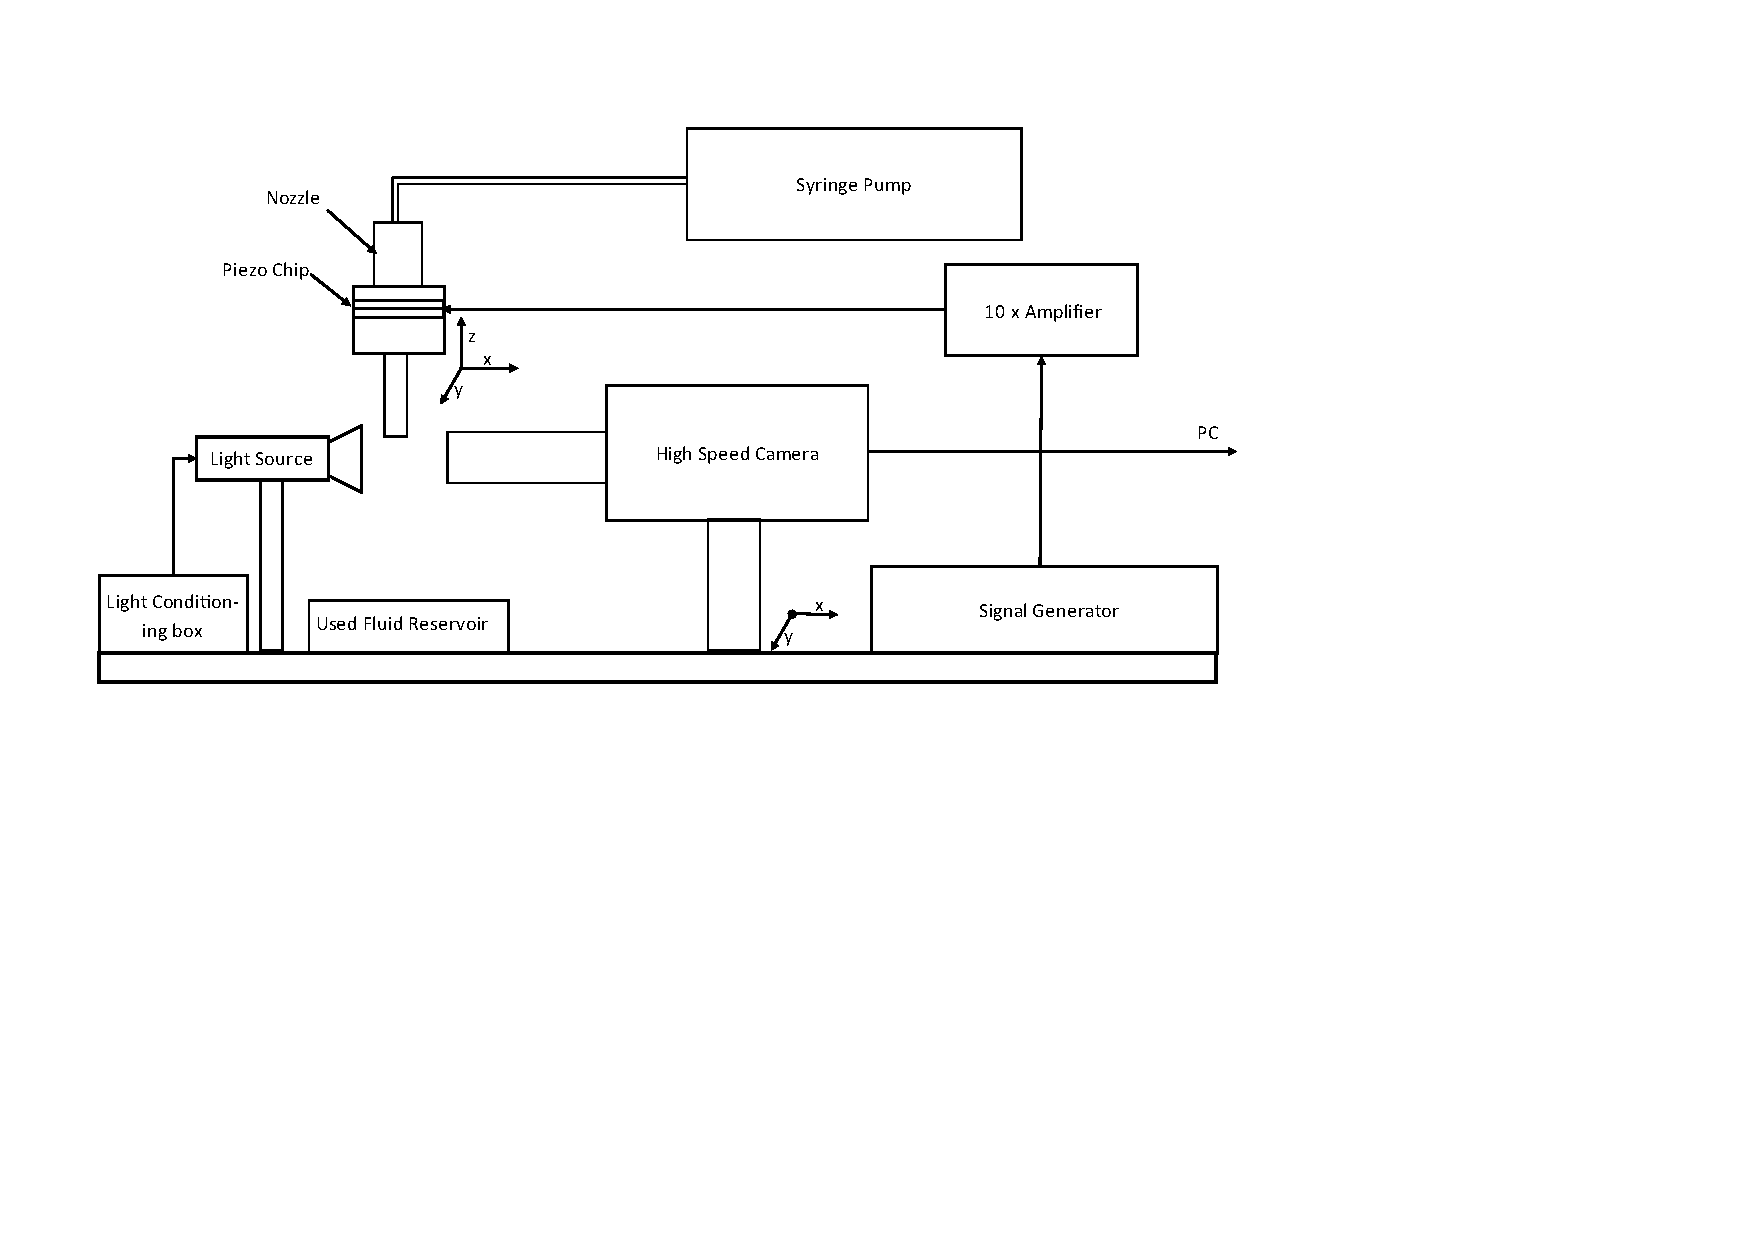
\includegraphics[trim=0cm 9cm 8cm 1.5cm, width = 0.7\textwidth]{img/ROJER_schematic.pdf}
	\caption{A schematic diagram of the ROJER setup. The liquid jet is 
perturbed by a piezoelectric actuator at the nozzle, with a driving frequency 
set by the signal generator. The motion of the jet is captured using a high 
speed camera. Graphic used with the permission of \cite{greiciunas2015report}}
	\label{fig:schematic}
\end{center}
\end{figure}

\subsubsection{Nozzle Designs} \label{sec:nozzles}

There are two needle designs for the nozzle that will be tested in order to 
determine their effect on the operating range of ROJER. Nozzle 1 is based on an 
orifice design with a nozzle diameter of $200 \mu m$ and is used to test 
Newtonian fluid materials only. This is due to concerns over potential flow 
blockages to the electron microscope aperture caused by testing viscoelastic 
fluids. This nozzle requires a stack of annular piezoelectric blocks (supplied 
by Thor Labs) surrounding the nozzle to drive the disturbance. The orifice 
design is assumed to exhibit a uniform jet exit velocity profile. Nozzle 1 is 
not cost effective and therefore the challenge is to test an alternative nozzle 
design.

The second nozzle is based on a disposable needle design. This is cheaper to 
manufacture in comparison to the first nozzle and relies upon two piezoelectric 
actuators clamped to the needle hub to provide the perturbation. The diameter 
of the hypodermic needle is $210 \mu m$ and the length of the nozzle is $4mm$. 
The length of this needle was selected using a laser microjet cutter and was 
chosen so that the pressure drop was small enough for the motor syringe pump to 
overcome. The advantage of this nozzle is that it is an ideal way of testing 
viscoelastic fluids owing to the disposable design. As a result of a CFD 
parameter study conducted by \cite{greiciunas2015report} is is expected the 
needle design exhibits a fully developed parabolic exit velocity profile.
\begin{figure}
	\centering
	\begin{subfigure}
		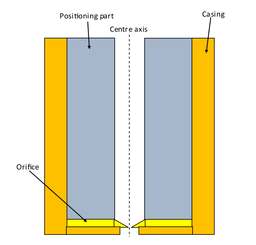
\includegraphics{img/old-nozzle_256_x_256.png}
		\caption{Needle 1 - the orifice design needle}
	\end{subfigure}
	\hfill
	\begin{subfigure}
		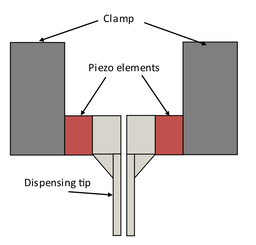
\includegraphics{img/new-nozzle_256_x_256.png}
		\caption{Needle 2 - the needle design needle}
	\end{subfigure}		
	\caption{The schematics of the ROJER tested nozzle designs, images courtesy 
of \cite{greiciunas2015report}}
\end{figure}

\subsubsection{Fluid Materials} \label{sec:materials}
For the fluid materials Newtonian and polymeric solutions are tested. Water and 
a water glycerol solution of a $60{\text -}40 \%$ volume concentration will be 
used to benchmark the tests and provide a comparison of the performance of each 
nozzle design as their Newtonian properties are well characterised. A more 
viscous water glycerol solution of a $24 {\text -} 76 \%$ concentration is 
tested in order to probe a higher Ohnesorge number parameter space. The 
extensional properties of ethyl hydroxy ethyl cellulose (EHEC) of molecular 
weight $M_w = 300 kg/kmol$ and poly ethylene oxide (PEO) of molecular weight 
$M_w = 250 kg/kmol$ are tested using the needle nozzle design and at different 
concentrations. This is typically be conducted at a flow infusion rate of 
$Q=5ml/min$ which is not independent of nozzle exit effects - see Section 
\ref{sec:exit} for further discussion. A table of physical properties for the 
fluids tested are given in Table 1. The surface tension $\gamma$ was measured 
using the Wilhelmy plate method. For water this was found to be $74 \, mPa \cdot 
s$, $62 \, mPa \cdot s$ for water glycerol $60 {\text -} 40\%$  and $62 \, mPa 
\cdot s$ also for water glycerol $24 {\text -} 76 \%$. The surface tension for 
the polymer solutions were all measured to be $62 \, mPa \cdot s$ which is the 
same as the solvent value. This is to be expected since surface tension is 
influenced only by the effects of intermolecular forces at the liquid-air 
interface, which is not altered by a colloidal suspension of the polymer. In 
general, increasing the amount of polymer added increases the zero shear 
viscosity $\mu_0$ of the solution and at higher shear rates the solution will 
approach the solvent viscosity, which is measured to be $\mu_{s} = 4.2 mPa \cdot 
s$.
\begin{table}[t]
\begin{center}
	\begin{tabular}{|c|c|c|c|c|c|} \hline
		\textbf{Test Fluid} & \textbf{Water wt. \%} & \textbf{Glycerol wt. \%} 
& \textbf{Polymer wt. \%} & $\mathbf{\mu \left(mPa\cdot s\right)}$ & 
$\mathbf{\rho \left( kg\cdot m^{-3} \right)}$  \\ \hline 
		Water & - & - &  - & 1.0 & 1,000 \\ 
		Water-Glycerol 60-40\% & 54.5 & 45.7 & - & 6.7 & 1,153 \\ 
		Water-Glycerol 24-76\% & 25.5 & 74.5 & - & 35.8 & 1,172  \\
		EHEC 0.1\% & 70.35 & 29.55 & 0.1 & 4.3 & 1,045 \\
		EHEC 0.2\% & 70.25 & 29.55 & 0.2 & 4.3 & 1,045  \\
		EHEC 0.4\% & 70.05 & 29.55 & 0.4 & 7.9 & 1,045  \\
		EHEC 0.6\% & 69.85 & 29.55 & 0.6 & 11.5 & 1,045 \\
		PEO 0.1\% & 70.35 & 29.55 & 0.1 & 3.6 & 1,045 \\ \hline
	\end{tabular}
	\label{tbl:fluid_prop}
	\caption{Physical properties of all test solutions measured at $20^\circ C$. 
Note the percentage concentration is given by weight rather than volume. The 
dynamic (shear) viscosity $\mu$ was obtained using the cone and plate geometry 
in a torsional rheometer.}
\end{center}	
\end{table}

The critical overlap concentration $c^*$ is a measure of ``diluteness" of a 
polymer solution. A widely accepted definition proposed by 
\cite{graessley1980polymer} is given by 
\begin{align}
c^* = \frac{0.77}{\left[ \mu \right]}
\end{align}
where $\left[ \mu \right]$ is the intrinsic viscosity. This is dependent on the 
polymer molecular weight $M_w$ through the Mark-Houwink expression
\begin{align}
\left[\mu \right] = 0.0072 M_w^{3 \nu - 1}
\end{align}
where the solvent quality parameter $\nu$ is 0.55 for EHEC and 0.56 for PEO 
\citep{keshavarz2015studying}, \citep{sharma2015rheology}. The longest 
relaxation time of a dilute polymer solution can be described by the Rouse Zimm 
model
\begin{align}
\tau_{Z} \sim \frac{\left[\mu \right] \mu_s M_w}{RT}
\end{align}
where $\mu_s$ is the solvent viscosity, $R$ is the ideal gas constant and $T$ 
is the temperature. It can be seen from this equation that the longest 
relaxation time is independent of the polymer concentration. For the test 
solutions EHEC 0.4, 0.6\% $c/c^* > O(1)$ and so these are therefore classed as 
semi dilute polymer solutions. \cite{tirtaatmadja2006drop} show that the Rouse 
Zimm model is in good agreement with higher values of $c/c^*$ since the 
dependency on the molecular weight remains similar. Thus the longest relaxation 
time for $M_w = 300 kg/kmol$ EHEC dispersed in a water-glycerol solution is 
predicted to be $\tau_{Z} = 135 \mu s$ and for PEO with $M_w = 250 kg/kmol$ the 
longest relaxation time is predicted to be $\tau_Z = 145 \mu s$. For a summary 
of the rheological properties of the polymeric solutions, please refer to Table 
\ref{tbl:rheo_prop}. 
\begin{table}[t]
\begin{center}
	\begin{tabular}{c|c|c|c|c|c|c|c} \hline
		\textbf{Test Fluid} & $\mathbf{M_w (kg/kmol)}$ & \textbf{c \%} & 
$\mathbf{c/c^*}$ & $\mathbf{\mu_0 (mPa \cdot s)}$ & $\mathbf{\tau_Z (\mu s)}$ & 
$\mathbf{De}$ & $\mathbf{Oh}$  \\ \hline 
		EHEC 0.1\% & 300 & 0.1 & 0.34 & 4.2 & 135 & 0.34 &0.04 \\
		EHEC 0.2\% & 300 & 0.2 & 0.68 & 4.2 & 135 & 0.34 &0.04 \\
		EHEC 0.4\% & 300 & 0.4 & 1.36 & 8.0 & 135 & 0.34 &0.07 \\
		EHEC 0.6\% & 300 & 0.6 & 2.04 & 11.5 & 135 & 0.34 &0.10 \\
		PEO 0.1\% & 250 & 0.1 & 0.44 & 6.9 & 145 & 0.37 & 0.03\\ \hline
	\end{tabular}
	\caption{Rheological properties of the viscoelastic test fluids at $20^\circ 
C$. Four different concentrations of ethyl hydroxy ethyl cellulose (EHEC) and 
one concentration of poly ethylene oxide (PEO) were dispersed in a Newtonian 
solvent (water ${\text -}$ glycerol), which has a solvent viscosity of $\mu_s = 
4.2 mPa \cdot s$. The zero shear viscosity $\mu_0$ measurements were made using 
a torsional rheometer.}
	\label{tbl:rheo_prop}
\end{center}	
\end{table}

\subsubsection{Exit Effects}
\label{sec:exit}
\cite{harmon1955drop} showed using a simple momentum balance for a laminar flow 
that the diameter of a jet downstream of the nozzle exit is a factor of 
$\sqrt{3}/2$ smaller than that of the nozzle diameter itself. This is because 
the shear stress exerted by the air on the free surface of the jet is 
negligible in comparison to the shear stresses experienced at the walls of the 
nozzle tube and so the fluid relaxes to a plug flow assuming there exists a 
fully developed a parabolic velocity profile at the exit.

However Harmon's analysis fails to account for the effect of surface tension 
which is significant at smaller Reynolds number, or for the effect of viscosity 
in which some of the kinetic energy of the jet will dissipate into heat. An 
even greater possible source of error however is the assumption that the flow 
achieves a parabolic profile right at the nozzle exit. Changes to the velocity 
profile can occur before the nozzle exit since the effects of vorticity 
produced by Kelvin Helmholtz instability at the jet interface can diffuse 
upstream into the nozzle.

\cite{goren1966shape} consider experimentally the expansion and contraction of 
a Newtonian jet downstream of the nozzle exit at different Reynolds numbers. 
Empirically they conclude that the critical Reynolds number to achieve a 
downstream diameter equal to the initial jet diameter is 14. Below this number 
the jet expands and above this number the jet contracts. For a flow infusion 
rate of $Q$ the resulting Reynolds number of the flow is defined as
\begin{align*}
Re = \frac{\rho V_j D_0 }{\mu} = \frac{\rho Q D_0 }{\mu A }
\end{align*}
where $V_j$ is the initial jet velocity, $D_0$ is the initial jet diameter, 
$\rho$ is the fluid density, $\mu$ is the dynamic viscosity and $A$ is the 
cross sectional area of the initial jet. A CFD parameter study exploring the 
effects of varying Reynolds number on jet contraction and expansion has been 
conducted by \cite{greiciunas2015report} and \cite{gorbatenko2015report}.

In light of this study, it is concluded a Reynolds number flow of 14 must be 
enforced when operating ROJER with Nozzle 2 in order to avoid the effects of 
jet contraction or expansion. An alternative is to conduct a frequency sweep to 
determine an adjusted critical wavelength which corresponds to the shortest 
break up length. This adjusted critical wavelength takes into account the 
effect of jet expansion or contraction and comparison to Nozzle 1 can therefore 
be preserved.

\subsubsection{Image Analysis} \label{sec:image_analysis}
A custom built program in MATLAB \textsuperscript{\textregistered} is used to 
post process the images captured by the high speed camera. The videos are 
stored in a lossless Tagged Image File Format (TIFF) in order to retain the 
maximum amount of image data from the camera. The program is also capable of 
post processing animations generated by CFD. These are stored in an MP4 video 
format at full high definition resolution.

A typical video captured consists of 16,000+ frames at a pixel resolution of 
$800 \times 104$ captured with an exposure time of $2 \mu s$. For each frame 
the image processing program begins by converting the picture from a grayscale 
to an 8-bit format. The edges of the fluid filament become clearly identifiable 
and so the pixel widths of the filament along the axial $z$ direction can be 
calculated. A Lagrangian element is then chosen travelling at jet speed $V_j$ 
in which the midfilament diameter evolution can be recorded with time - see 
Figure \ref{fig:image_analysis}. Once this Lagrangian element reaches the 
position of jet break up, the process restarts and another collection of 
thinning jet diameters is made. Over $500$ collections of diameters are made in 
each video and so these are time averaged by placing the collections of 
diameters at a common break up time $t_b$. The conversion from frames to time 
is computed using the camera speed and the conversion from pixels to metres is 
computed using the initial jet diameter $D_0$. This process yields the overall 
evolution of the thinning midfilament diameter $D(t)$.
\begin{figure}
	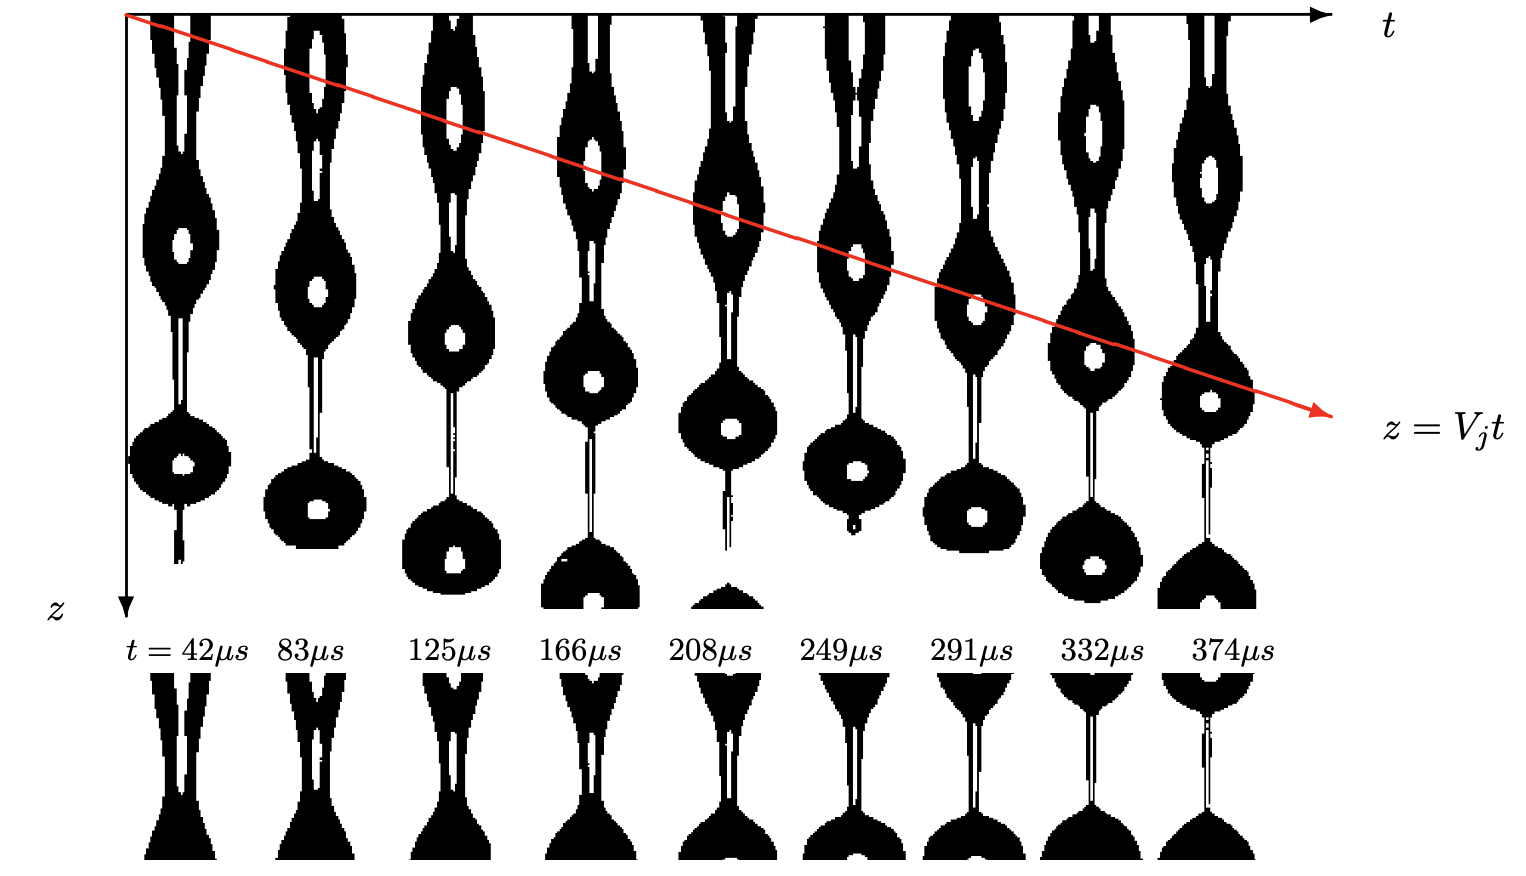
\includegraphics{img/image_analysis.png}
	\caption{(Above) A montage of images of the a weakly viscoelastic jet 
captured using ROJER. (Below) The thinning midfilament diameter in a Lagrangian 
element of the jet moving at a jet speed of $V_j$.}
	\label{fig:image_analysis}
\end{figure}

\subsection{Operation}
By understanding the dynamics of capillary driven jet break up, ROJER can be 
used as an extensional rheometer in order to characterise the extensional 
properties of dilute polymer solutions.

As described in Section \ref{sec:stability}, it is expected that the initial 
Rayleigh-Plateau instability in the linear region of the jet will follow a 
midfilament diameter evolution of
\begin{align}
\frac{D(t)}{D_0} = 1 - \delta \exp (\alpha t)
\label{eqn:linear_region}
\end{align}
where $\delta$ is the ratio of the initial perturbation amplitude to the 
initial jet diameter ($\delta = \delta_0 / D_0$) and $\alpha$ is the growth 
rate according to the dispersion relation in Equation \ref{eqn:dispersion_viscous} 
for viscous jets and Equation \ref{eqn:dispersion_viscoelastic} for viscoelastic 
jets.

As the instability grows, the strain rate $\dot{\epsilon}$ increases and the 
decreasing midfilament diameter $D(t)$ no longer adheres to Equation 
\ref{eqn:linear_region} due to significant resistance from viscoelastic 
stresses, resulting in a slower decay of $D(t)$. For Newtonian fluids, 
transition to the viscocapillary regime occurs when the viscous timescale 
$\left(t_{vis} = \mu D(t) /\gamma \right)$ divided by the inertial (Rayleigh) 
timescale $\left(t_R = \sqrt{\rho D(t)^3}/\gamma \right)$ becomes the order of 
unity \citep{clasen2012dispensing}
\begin{align*}
Oh = \mu/\sqrt{\rho D(t)^3 \gamma} \sim O(1).
\end{align*}
For polymeric fluids, transition to the elastocapillary regime occurs when the 
local Deborah number, which is the ratio of the polymer relaxation time to the 
inertia capillary timescale, is of order one 
\begin{align*}
De = \tau_E / \sqrt{\rho D(t)^3/\gamma} \sim O(1).
\end{align*}
Here the thinning midfilament diameter of an Oldroyd B fluid follows Equation 
\ref{eqn:elasto_thinning}
\begin{align}
\frac{D(t)}{D_0} = \left(\frac{G D_0}{4 \gamma}\right)^{1/3} \exp 
\left(\frac{-t}{3 \tau_E}\right),
\label{eqn:elasto_thinning4}
\end{align}
and so by fitting this equation to the data $D(t)$ in the elastocapillary 
thinning obtained by ROJER, it is possible to obtain the relaxation time 
$\tau_E$ of the fluid.

The evolution of the thinning midfilament diameter $D(t)$ of a forced jet 
issued by ROJER is also the key factor to determining the transient extensional 
viscosity $\mu_E$ at an instantaneous strain rate $\dot{\epsilon}$. This is 
given by the expressions
\begin{align}
\dot{\epsilon} &= \frac{2}{D(t)} \od{D(t)}{t} \label{eqn:strain_rate} \\
\mu_E &= \frac{- \gamma}{d D(t) / dt} \label{eqn:ext_viscosity}
\end{align}
as outlined by \cite{anna2001elasto}.

\subsection{Reproducibility} \label{sec:reproducibility}
The output $D(t)$ can vary significantly depending on the wavenumber of the jet 
perturbation, especially given the unknown exit effects of Nozzle 2. It is 
therefore appropriate to validate the experimental results of ROJER with the 
expected growth rates outlined in Section \ref{sec:stability}.
\begin{figure}[h]
	\begin{subfigure}
		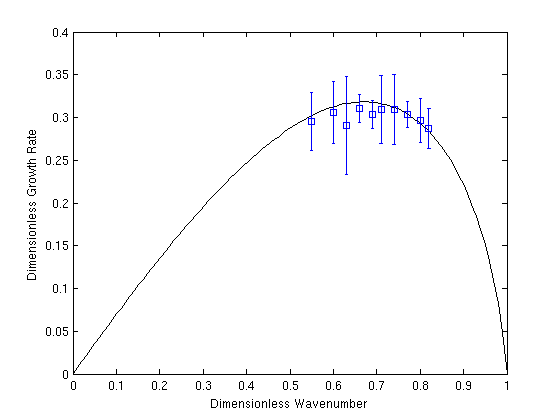
\includegraphics[scale=0.5]{img/sweep4.png}
		\caption{The dimensionless wavenumber against the dimensionless growth 
rate for EHEC 0.4 wt.\% using Nozzle 2 $\left(Oh = 0.07, We = 20.5 \right)$. 
The predicted growth rate derived from the linear theory is plotted as a solid 
black line and the observed growth rate is denoted by the blue squares.}
	\end{subfigure} \hfill
	\begin{subfigure}
		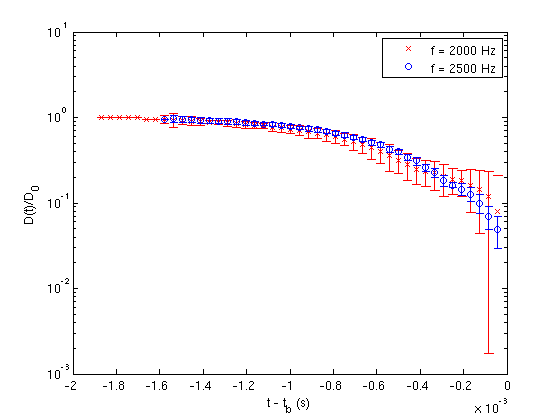
\includegraphics[scale=0.5]{img/sweep7.png}
		\caption{The normalised jet midfilament diameter $D(t)/D_0$ for EHEC 
wt.\% $\left(Oh = 0.07, We = 20.5 \right)$. The jet is perturbed at apparent 
critical frequency $f = 2,500 Hz$ corresponding to the most amplified growth 
rate, and a lower frequency $f = 2,000 Hz$ corresponding to a wavenumber lower 
than the critical.}
	\end{subfigure}
	\caption{These graphs demonstrate a narrow band of wavenumbers between the 
most unstable one and the margin of stability is required to operate ROJER 
effectively. For Nozzle 2 these wavenumbers must be adjusted for empirically 
given jet contraction or expansion effects.}
	\label{fig:sweep7}
\end{figure}

In Figure \ref{fig:sweep7} (a), the growth rate $\alpha$ and the initial 
perturbation amplitude $\delta$ are determined by fitting a function of the 
form specified by Equation \ref{eqn:linear_region} to the linear region of the 
jet for each wavenumber tested. The theoretical growth rate is plotted also for 
comparison using the viscoelastic dispersion relation 
\ref{eqn:dispersion_viscoelastic}. This shows that the predicted values of the 
growth rate agree very well with the experimental values obtained using Nozzle 
2, therefore ROJER is quite well described by the linear theory despite the 
nozzle exit effects. The theoretical critical wavenumber is calculated to be 
$k^*R_0 = 0.7$ and it can be seen that the optimal operation of ROJER lies in 
the narrow band of wavenumbers between the most unstable one and the margin of 
stability, i.e. $k^* R_0 \leq k R_0 \leq 1$.

As mentioned in Section \ref{sec:image_analysis} over $500$ collections of 
diameters are made in each video, in which $D(t)$ is determined by placing all 
collections at a common zero and taking a time average. Another measure of the 
reproducibility of the results is to evaluate the standard error of the 
collections of diameters, for a 0.4 wt.\% EHEC solution at varying frequencies 
using Nozzle 2. Figure \ref{fig:sweep7} (b) shows the results of two such 
frequencies during a frequency sweep, in which the apparent critical frequency 
$f = 2,500$ accounts for presumed jet contraction and $f = 2,000$ corresponds 
to a lower wavenumber disturbance. The observations demonstrate that the 
optimal operating range for ROJER using Nozzle 2 improves if the perturbation 
wavenumber is closer to the apparent critical wavenumber corresponding to the 
most amplified growth rate. This is in agreement with the numerical results of 
\cite{ardekani2010dynamics}, where it was shown that the optimal range for 
extensional rheometry coincides with the absence of satellite drops. 
Preliminary experiments with ROJER have shown that weakly viscoelastic jets can 
generate satellite drops at low wavenumber perturbations, which diminish in 
size as the wavenumber approaches the apparent critical wavenumber. These 
satellite drops vanished at wavenumbers beyond this critical wavenumber but 
less than the margin of stability due to the enhanced stability provided by the 
polymers - see Figure \ref{fig:satellite}. 

In conclusion the effective operation of ROJER is achieved between the critical 
wavenumber and the margin of stability $k^* R_0 \leq k R_0 \leq 1$. It is 
required that this range must be adjusted for empirically when using Nozzle 2 
due to nozzle exit effects.
\begin{figure}[h]
	\begin{subfigure}
		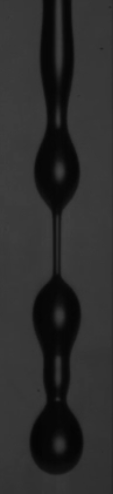
\includegraphics[scale=0.25, trim = 0cm 0cm 0cm 2.1cm, clip = 
true]{img/less_critical.png}
	\end{subfigure} \hfill
	\begin{subfigure}	
		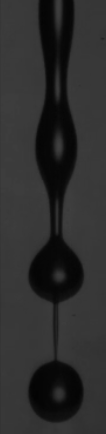
\includegraphics[scale=0.25]{img/more_critical.png}
	\end{subfigure}
	\caption{(a) Wavenumbers below the most unstable wavenumber $kR_0 < k^* R_0$ 
lead to the formation of satellite drops which merge with the leading drop. (b) 
Wavenumbers above the most unstable wavenumber suppresses the appearance of 
satellite drops and a stable beads on a string morphology is seen.}
	\label{fig:satellite}
\end{figure}

\newpage

\section{Results and Discussion}
An operating range with respect to varying Ohnesorge and Weber numbers is 
established. A comparison is then made between the two different nozzle designs 
using water${\text -}$glycerol to benchmark the test. A small study evaluating 
measured jet break up lengths is used to estimate the amplitude of the initial 
jet perturbation. Finally the extensional properties of EHEC and PEO are 
extracted using ROJER.

\subsection{Operating Range} \label{sec:operating}
An operating range for ROJER is established by varying the Ohnesorge and Weber 
numbers of the jet. Recall
\begin{align}
Oh = \frac{\mu}{\sqrt{\rho \gamma D_0}} \hspace{2cm} We = \frac{\rho V_j^2 
D_0}{\gamma}
\end{align}
where $\mu$ is the dynamic viscosity of the fluid, $\rho$ is the density, 
$\gamma$ is the surface tension, $D_0$ is the initial jet diameter and $V_j$ is 
the velocity of the jet. Variation of these dimensionless parameters can be 
achieved through controlling the flow rate, fluid material and the 
implementation of the two different nozzle designs. The operating map for 
Newtonian fluids is presented in Figure \ref{fig:operability}.
\begin{figure}[h]
	\begin{center}
		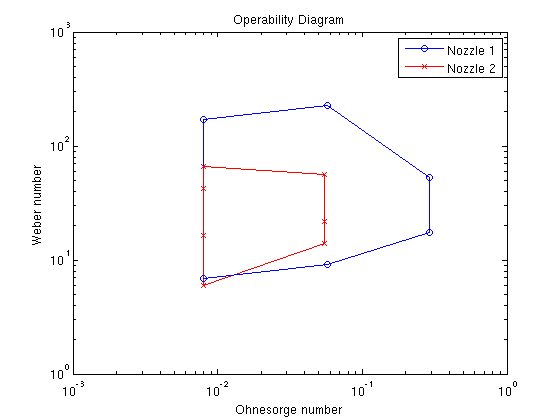
\includegraphics[scale=0.5]{img/operability.png}
		\caption{An operability diagram for ROJER showing the minimum and 
maximum Ohnesorge and Weber numbers required for the successful operation of 
the device.}
		\label{fig:operability}
	\end{center}
\end{figure}
The operating space for the needle design nozzle (Nozzle 2) is much more 
limited in scope than for the orifice design nozzle (Nozzle 1). A summary of 
minimum and maximum values of the dimensionless parameters for each nozzle are 
presented in Table \ref{tbl:operability}. 
\begin{table}[h]
\centering
\begin{tabular}{c|c|c|c|c|}
\cline{2-5}
                               & $Oh_{min}$ & $Oh_{max}$ & $We_{min}$ & 
$We_{max}$ \\ \hline
\multicolumn{1}{|c|}{Nozzle 1} & 0.008      & 0.293      & 6.90       & 228.70 
    \\ \hline
\multicolumn{1}{|c|}{Nozzle 2} & 0.008      & 0.055      & 5.95       & 66.2    
   \\ \hline
\end{tabular}
\caption{A table of values for the limits of the Ohnesorge and Weber for the 
two different nozzle designs.}
\label{tbl:operability}
\end{table}

\subsection{Nozzle Comparison}
To compare the performance of the two nozzle designs, see Section 
\ref{sec:nozzles}, they will be used to characterise the properties of 
Newtonian fluids using ROJER. Their expected behaviour is validated using a one 
dimensional model by \cite{hall2015report} and the Volume of Fluid (VOF) method 
in ANSYS Fluent by \cite{greiciunas2015report} and in STAR-CCM+ 
\citep{gorbatenko2015report}.

Water and a water-glycerol $60 {\text -} 40 \%$ solution is tested. The 
frequency is controlled so that the most amplified growth rate is selected - 
see Section \ref{sec:reproducibility}. The Ohnesorge numbers for water and 
water-glycerol $60 {\text -} 40 \%$ are $0.008$ and $0.056$ respectively and 
can therefore be approximated as inviscid fluids. Using the longwave 
approximation to the dispersion relation (Equation \ref{eqn:dispersion_longwave}) 
the critical wavenumber, wavelength and frequency  resulting in the most 
amplified growth rate can therefore be calculated. A table summarising these 
experimental parameters plus dimensionless numbers are presented in Table 
\ref{tbl:exp_1}.
\begin{table}[h]
\centering
\begin{tabularx}{\textwidth}{c *{7}{|Y}|}
\cline{2-7}
& Wavenumber & Wavelength (mm) & Frequency (Hz) & Ohnesorge number  & Reynolds 
number & Weber number \\ \hline
\multicolumn{1}{|c|}{Water}                              & 0.70       & $0.90$   
  & 2,949     & 0.008 & 531  & 19   \\ \hline
\multicolumn{1}{|c|}{Water-Glycerol $60 {\text -} 40 \%$} & 0.65       & $0.96$   
  & 2,762     & 0.056 & 91   & 26   \\ \hline
\end{tabularx}
\caption{The critical experimental parameters and dimensionless numbers imposed 
on the Newtonian test fluids to compare the nozzle designs. Note that the 
dimensionless numbers are computed using the initial jet diameter $D_0$. These 
parameters correspond to the most amplified growth rate.}
\label{tbl:exp_1}
\end{table}

As outlined by the linear stability theory, it is expected that increasing 
viscosity increases the length of the most unstable wavelength. A flow rate of 
$Q = 5ml/min$ results in a very high Reynolds number flow for water in 
comparison to water-glycerol $60 {\text -} 40 \%$ therefore nozzle exit effects 
in Nozzle 2 may be more pronounced in the case for water - see Section 
\ref{sec:exit}. Graphs of the evolution of the thinning diameters for water and 
water-glycerol $60 {\text -} 40 \%$ are presented in Figure \ref{fig:flat_vs_para}.
\begin{figure}[h]
	\begin{subfigure}
		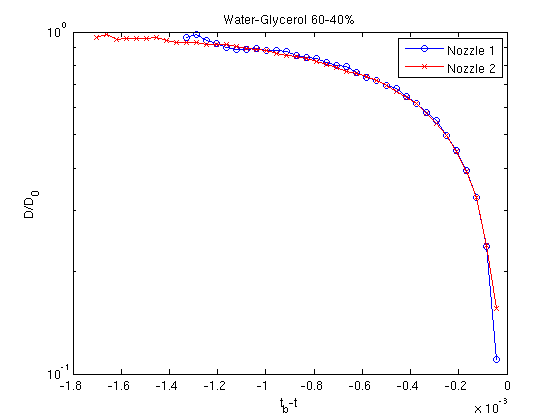
\includegraphics[width = 0.55 \textwidth]{img/water-glycerol_flat_vs_para(2).png}
	\end{subfigure}
	\begin{subfigure}
		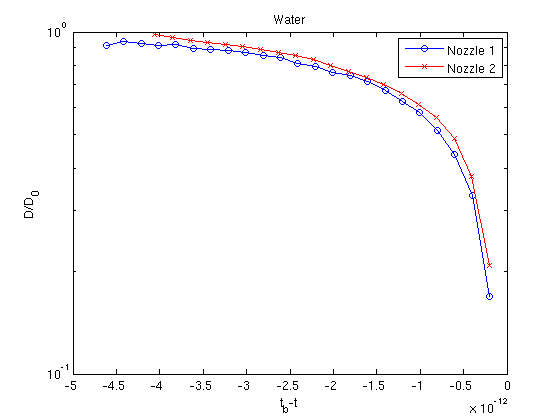
\includegraphics[width = 0.55\textwidth]{img/water_flat_vs_para(2).png}
	\end{subfigure}
\caption{(a) The thinning midfilament diameter of a water and (b) 
water-glycerol $60 {\text -} 40 \%$ jet over time.}
\label{fig:flat_vs_para}
\end{figure}

A paired difference t-test is used to determine whether the impact of changing 
from Nozzle 1 to Nozzle 2 is significant in the case for water and for 
water-glycerol $60 {\text -} 40 \%$. A significance level of $5\%$ is selected. 
The mean difference $\bar{d}$ is calculated
\begin{align*}
\bar{d} = \frac{1}{n} \sum^n_{i=1} \left(D_{i2} - D_{i1} \right)
\end{align*}
where $n$ is the number of paired samples, and $D_{i1}$ and $D_{i2}$ are the 
collections of diameters for Nozzle 1 and Nozzle 2 respectively. The standard 
deviation of the differences $s$ are then computed. The t-statistic is given by
$T = \bar{d}/s$. Under the null hypothesis this follows a two tailed 
t-distribution with $n-1$ degrees of freedom. For water-glycerol $T = 0.294$ 
which is less than the p-value of $2.037$, therefore the null hypothesis is 
accepted and so the use of Nozzle 2 has no significant difference to the use of 
Nozzle 1 for a significance level to $5 \%$. For water $T = 2.643$ and is 
greater than the p-value of $2.086$, therefore the null hypothesis is rejected 
and so the use of Nozzle 2 does have a significant impact on the results. It 
can be speculated this could possibly be due to increased nozzle exit effects 
experienced at the higher Reynolds number flow for water. 

\cite{greiciunas2015report} was able to determine the rate of 
contraction/expansion in nozzle 2 by comparing the observed wavelength of the 
jet to the expected wavelength based upon the driving frequency. The apparent 
velocity and therefore in turn the Reynolds number of the flow can be inferred, 
whilst the downstream jet diameter is calculated through mass conservation. 
Experimental results of the Newtonian fluids are within acceptable limits of 
the data obtained by \cite{middleman1961expansion} however viscoelastic 
experiments do not compare well. This study may be limited by the pixel 
resolution of the images obtained from ROJER - see Section \ref{sec:error}.

\subsection{Jet Break Up Lengths} \label{sec:exp_breakup}
Recall in Section \ref{sec:breakup_length} an expression was derived to predict 
the critical break up length of a linear inviscid jet
\begin{align}
\frac{L^*}{D_0} = 3C \, \mathrm{We}^{1/2},
\label{eqn:inviscid_breakup}
\end{align}
where $C = \ln \left( D_0 / \delta  \right)$ denotes the unknown ratio between 
the initial diameter of the jet $D_0$ and the amplitude $\delta$ of the initial 
perturbation $\tilde{\delta} = \delta_0 \exp (ikz + \alpha t)$. It should be 
noted the Weber number is based on the initial jet diameter $D_0$. 

By measuring the critical break up lengths $L^*$ of the Newtonian test fluids 
using Nozzle 1, it is possible to experimentally determine the unknown 
parameter $\delta$. The Ohnesorge number of these flows are much less than one, 
therefore an inviscid approximation is implemented. The break up lengths are 
measured using a vernier caliper mounted beside the jet. The results are 
presented in Figure \ref{fig:breakup}.
\begin{figure}[h]
\centering
	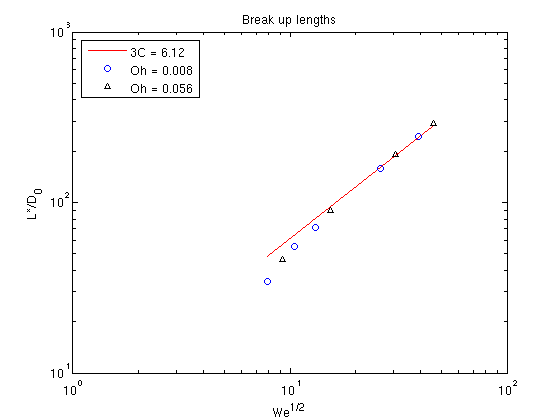
\includegraphics[width = 0.5 \textwidth]{img/breakup.png}
	\caption{The experimental dimensionless critical break up lengths $L^*/D$ 
fitted with Equation \ref{eqn:inviscid_breakup}. This gives an approximate jet 
perturbation amplitude of $\delta/D_0 \approx 0.22$.}
	\label{fig:breakup}
\end{figure}

The Weber number was varied by adjusting the flow rate $Q$, and two Ohnesorge 
numbers were evaluated using water and water-glycerol $60 {\text -} 40 \%$ as 
test solutions. It can be seen by fitting Equation \ref{eqn:inviscid_breakup} 
to the data that the experiments yield a value of $C =2.04$. The initial 
perturbation amplitude is therefore computed to be $\delta = 4.4 \times 10^{-7} 
m$ which is $22\%$ of the initial jet diameter $D_0$. This observation is much 
greater than the specified perturbation amplitudes used in the one dimensional 
and CFD simulations. Potential limitations of this experiment are discussed in 
Section \ref{sec:error}. 

\subsection{Viscoelastic Fluids}

\subsubsection{EHEC Concentrations 0.1, 0.2, 0.4 and 0.6 wt.\%} \label{sec:EHEC}
EHEC solutions with weight concentrations $c=0.1$, 0.2, 0.4 and 0.6 wt.\% were 
tested using Nozzle 2 (needle design). A voltage of $10V$ and a constant flow 
rate of $Q = 5ml/min$ was applied. The jet is perturbed at a driving frequency 
corresponding to the most amplified growth rate $\alpha^*$, which is determined 
empirically through conducting a frequency sweep to identify the critical 
(shortest) break up length.

As discussed in Section \ref{sec:materials}, the predicted Zimm relaxation time 
was found to be $\tau_{Z} = 135 \mu s$, which is independent of the polymer 
concentration. Plots of $D(t)/D_0$ for concentrations 0.1 and 0.2 \% are 
presented in Figure \ref{fig:1_2_EHEC}, where the time axis is translated by 
the break up time $t_b$.
\begin{figure}[h]
	\begin{center}
		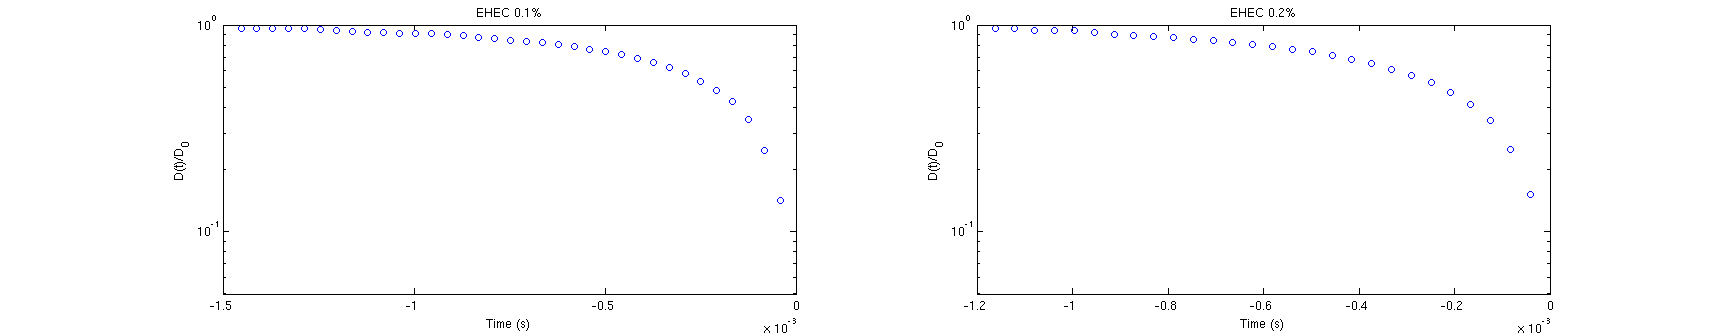
\includegraphics[scale = 0.45, trim = 7cm 0cm 6cm 0cm]{img/1_2_EHEC.png}
		\caption{The normalised thinning midfilament diameters of EHEC 0.1 and 
0.2 wt.\% $ \left(Oh = 0.037 , We = 20.5, Re = 123 \right)$. The expected 
exponential elastocapillary thinning regime cannot be observed, which could be 
due to insufficient camera speed.}
		\label{fig:1_2_EHEC}
	\end{center}
\end{figure}

It can be concluded that ROJER was not capable of capturing the elastocapillary 
region using the current setup for these polymer concentrations. The limit of 
the camera speed was $24,096$ frames per second, which is insufficient to 
provide the time resolution to observe the effect of the polymers uncoiling in 
the elastocapillary region. It is possible that the Ohnesorge number of $Oh = 
0.037$ is so low that the viscous forces could not overcome the fluid inertia 
for the viscoelastic stresses to prevail over the capillary forces. However the 
Ohnesorge number does not provide a full picture of the dynamics as it accounts 
for inertia, viscosity and surface tension only. It is therefore appropriate to 
evaluate the instantaneous strain rate using Equation \ref{eqn:strain_rate} to 
determine whether the flow evolves into a uniaxial extension of sufficient 
magnitude, which is presented in Figure \ref{fig:1_2_EHEC_strain}. 
\begin{figure}[h]
	\begin{center}
		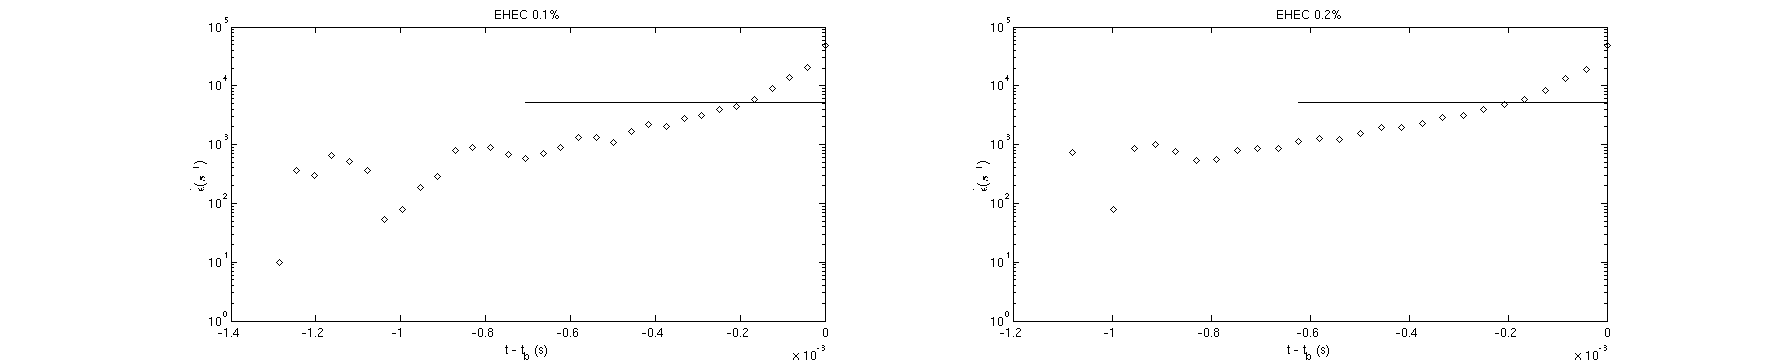
\includegraphics[width=0.95\textwidth, trim = 7cm 0cm 6cm 0cm]{img/1_2_EHEC_strain.png}
		\caption{The strain rate $\dot{\varepsilon}$ over time for EHEC 0.1 and 
0.2 wt.\%}
		\label{fig:1_2_EHEC_strain}
	\end{center}
\end{figure}

As detailed in Section \ref{sec:elasto} it is expected the instantaneous strain 
rate should plateau at a value approaching $Wi = 2/3$ during elastocapillary 
thinning, which is indicated by the solid line in Figure 
\ref{fig:1_2_EHEC_strain}. It can be clearly confirmed that this has not been 
achieved in the cases for 0.1 and 0.2 wt.\% EHEC as there is no evidence of 
such a plateau, and so the polymer coil to stretch transition has not been 
observed.

The plot of $D(t)/D_0$ for concentrations 0.4 and 0.6 wt.\% are presented in 
Figure \ref{fig:4_6_EHEC}. Regression of Equation \ref{eqn:elasto_thinning4} to 
the data in the elastocapillary region is also plotted as a solid red line.
\begin{figure}[H]
	\begin{center}
		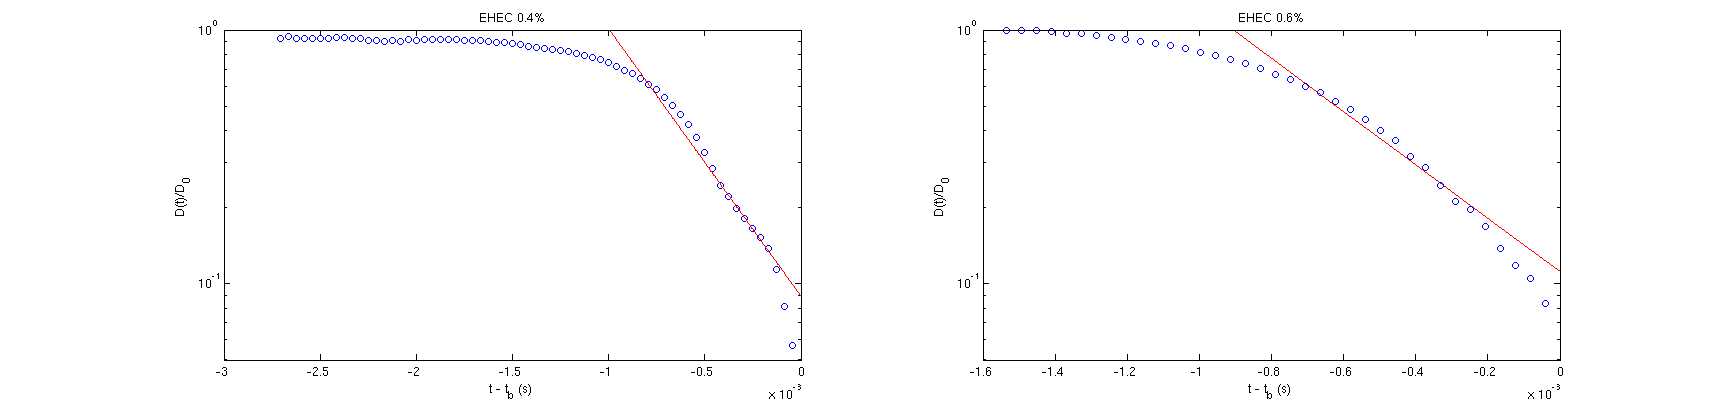
\includegraphics[width=0.95\textwidth, trim = 7cm 0cm 6cm 0cm]{img/4_6_EHEC.png}
		\caption{The normalised thinning midfilament diameters of EHEC 0.4 and 
0.6 wt.\% $ \left(Oh = 0.037 , We = 20.5, Re = 123 \right)$. Regression of the 
data in the elastocapillary region is plotted as a solid red line.}
		\label{fig:4_6_EHEC}
	\end{center}
\end{figure}

It is evident that ROJER has indeed captured the elastocapillary regime for 
these solutions given the exponential thinning observed. In addition it is 
possible to observe the transition from the elastocapillary regime to the 
viscocapillary regime for EHEC 0.4 wt.\%, which is evidenced by the linear 
decay observed in the final approach to break up as the polymers achieve 
maximum elongation. For 0.4 wt.\% EHEC the relaxation time was found to be 
$\tau_E = 137 \mu s$ and for 0.6 wt.\% EHEC $\tau_E = 138 \mu s$. These values 
are in good agreement with the predicted Zimm relaxation time of $\tau_{Z} = 
135 \mu s$, especially given the validity of the Rouse Zimm model for 
semi-dilute polymer solutions discussed in Section \ref{sec:materials}. The 
relaxation times observed here by ROJER also show that they are independent of 
the polymer concentration where the molecular weight and solvent viscosity is 
controlled. The strain rate of the flow was also evaluated and the results 
are presented in Figure \ref{fig:4_6_EHEC_strain}.
\begin{figure}[H]
	\begin{center}
		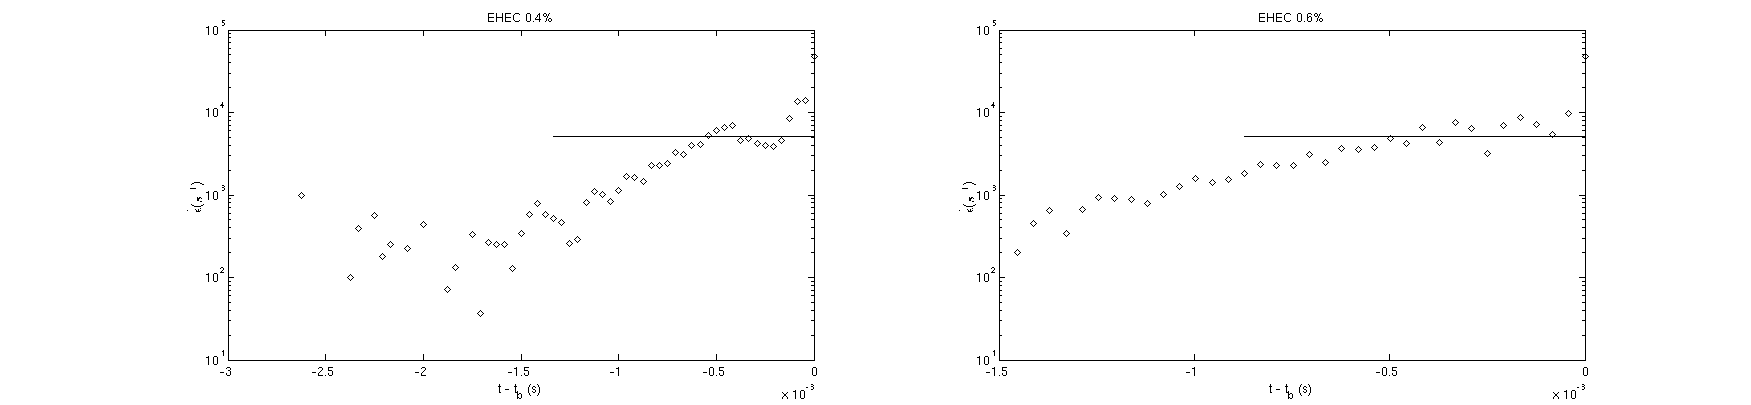
\includegraphics[width=0.95\textwidth, trim = 7cm 0cm 6cm 0cm]{img/4_6_EHEC_strain.png}
		\caption{The instantaneous strain rate $\dot{\varepsilon}$ over time 
for EHEC 0.4 and 0.6 wt.\%}
		\label{fig:4_6_EHEC_strain}
	\end{center}
\end{figure}

In contrast to the instantaneous strain rates computed for 0.1 and 0.2 wt.\%, 
the data here shows a plateau at a critical strain rate equivalent to $Wi = 
2/3$. This confirms that elastocapillary thinning was indeed achieved by ROJER 
and the regression of Equation \ref{eqn:elasto_thinning4} is valid.

Graphs of the transient extensional viscosity extracted from the jet thinning 
dynamics $D(t)$ via Equation \ref{eqn:elasto_thinning} are presented in Figure 
\ref{fig:EHEC_extensional}. It is difficult to measure a well defined 
extensional viscosity here since the data from ROJER has been restricted to the 
last stages of thinning.
\begin{figure}[h]
\begin{subfigure}
	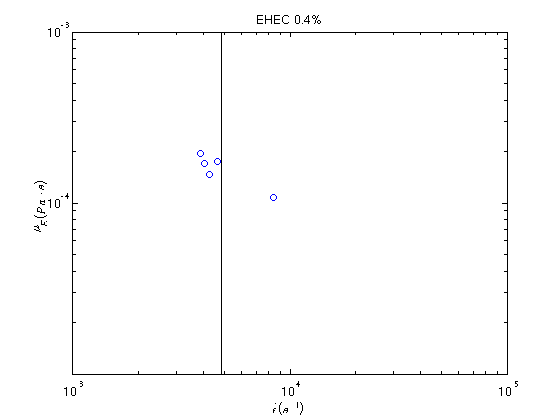
\includegraphics[width = 0.4\textwidth]{img/4_EHEC_extensional.png}
\end{subfigure} \hfill
\begin{subfigure}
	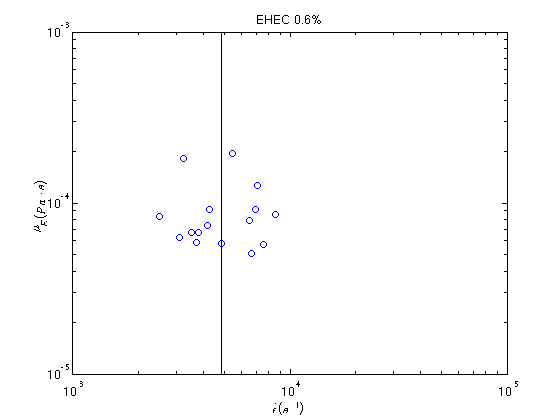
\includegraphics[width = 0.4 \textwidth]{img/6_EHEC_extensional.png}
\end{subfigure}
\caption{The transient extensional viscosity $\mu_E$ data of EHEC 0.4 and 0.6 
wt.\%. It is difficult to extract a well defined extensionanal viscosity here 
due to the limited dataset. }
\label{fig:EHEC_extensional}
\end{figure}

\subsubsection{PEO Concentration 0.1 wt.\%}
A PEO solution with a weight concentration of 0.1 wt.\% was also tested using 
Nozzle 2 (needle design). In similar conditions to EHEC, a voltage of $10V$ and 
a constant flow rate of $Q = 5ml/min$ was implemented at a driving frequency 
set to promote the most unstable wave mode.

In Section \ref{sec:materials} it was predicted the Zimm relaxation time was 
$\tau_Z = 145 \mu s$ for PEO. The evolution of the thinning midfilament 
diameter obtained by ROJER is presented in Figure \ref{fig:PEO}.
\begin{figure}[H]
	\begin{center}
		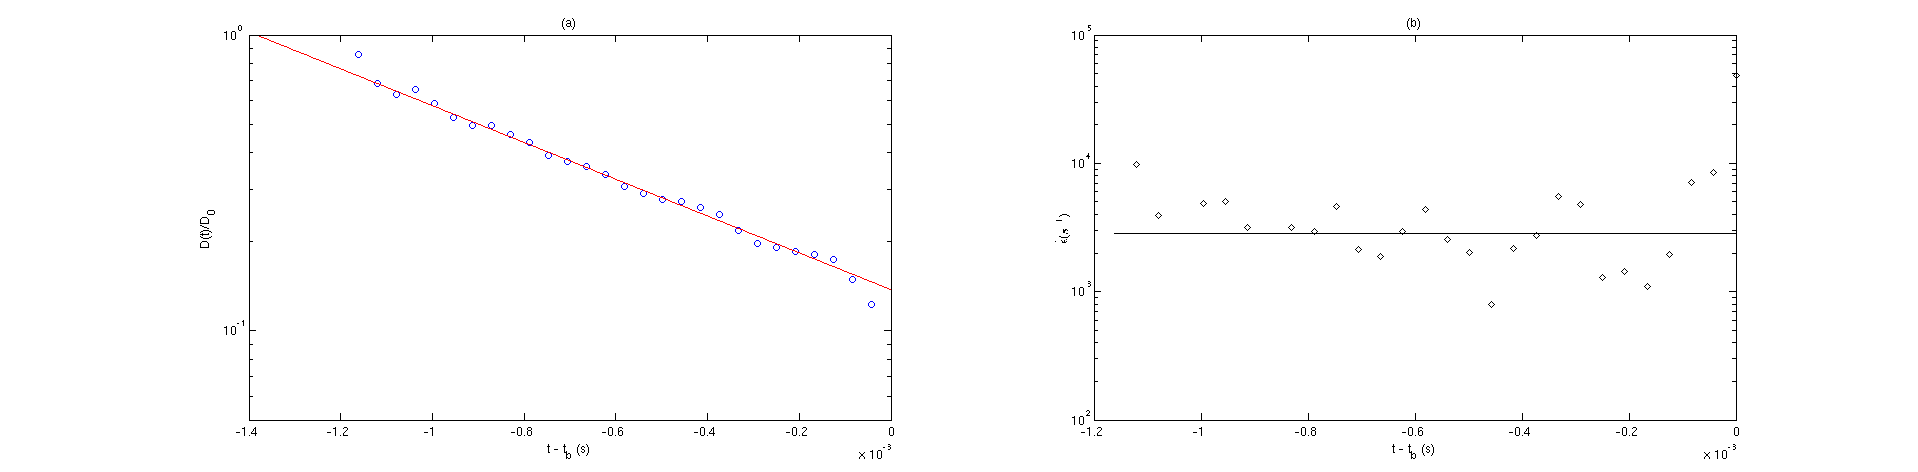
\includegraphics[width = 1.15\textwidth, trim = 6cm 0cm 0cm 0cm]{img/PEO.png}
		\caption{(a) The normalised thinning midfilament diameter $D(t)/D_0$ of 
PEO 0.1 wt.\%. Only elastocapillary thinning has been captured. (b) The 
instantaneous strain rate $\dot{\varepsilon}$ over time for PEO 0.1 wt.\%. All 
values deviate about the critical strain rate.}
		\label{fig:PEO}
	\end{center}
\end{figure}

Figure \ref{fig:PEO} (a) shows that given the $800 \times 104$ pixel resolution 
of the image, the linear region of the jet was unobservable and ROJER was able 
to capture the elastocapillary region only. By regression of the data to 
Equation \ref{eqn:elasto_thinning4} the relaxation time was determined to be 
$\tau_E = 233 \mu s$. This is significantly different from the predicted Zimm 
relaxation time, which could suggest the window of data captured was not 
representative of the elastocapillary thinning process due to the limited 
camera resolution, or that the Rouse Zimm model is not valid in this case. 
Figure \ref{fig:PEO} (b) shows the evolution of the instantaneous strain rate 
$\dot{\varepsilon}$, in which most of the data points deviate about the 
critical strain rate. 
\begin{figure}[h]
	\begin{center}
		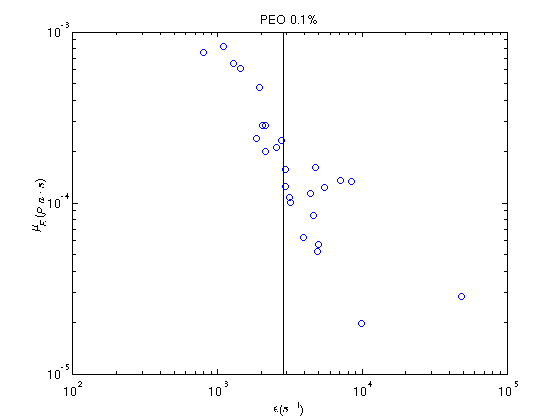
\includegraphics[width = 0.4\textwidth]{img/PEO_extensional.png}
		\caption{The transient extensional viscosity $\mu_E$ of 0.1 wt.\% PEO. 
Here there is evidence of strain hardening characteristics.}
		\label{fig:PEO_extensional}
	\end{center}
\end{figure}

The transient extensional viscosity presented in Figure 
\ref{fig:PEO_extensional} shows that PEO exhibits some appreciable strain 
hardening characteristics. Analysis of the instantaneous strain rate shows that 
a consistent plateau was not attained and a steady flow was not achieved, which 
may have significantly affected the fluid response to the flow. It is also 
worth noting that in theory the polymer is assumed to be monodispersed 
throughout the solution with a constant molecular weight, when in reality this 
not necessarily true despite careful preparation of the solutions. The 
molecular weight is in fact a distribution and the average is given by the 
supplier.

\subsection{Error Analysis} \label{sec:error}
Following the results and discussion, it can be concluded that using ROJER as 
an extensional rheometer has its limitations as with any other measuring 
device. Given the ROJER setup is a new technique, it is important to address 
these limitations in order to aid further development of this design. A survey 
of the accuracy and precision of the system is therefore conducted in this 
section.

It has been clearly identified in Section \ref{sec:EHEC} that image quality 
issues have a significant impact on the operation of ROJER. This in particular 
was highlighted in the tests for the 0.1 and 0.2 wt.\% EHEC solutions in which 
the elastocapillary thinning regime was not possible to image. The Phantom 
camera was required to capture images at a high frame rate at a high 
magnification with a very short exposure time, which led to low resolution 
images and poor illumination. A possible solution to this problem is to image 
the jet stroboscopically, as employed by \cite{keshavarz2015studying}, where 
the light source is strobed at very short and bright light pulses. This can be 
synchronised close to the driving frequency of the jet perturbations which 
results in an apparent slow motion effect up to a factor of $60,0000 \times$ 
slower. A high resolution digital camera can then instead be used to capture 
sharper images, providing access to the visualisation of the break up process. 
This would also aid in the evaluation of the transient extensional viscosity by 
increasing the number of samples in the elastocapillary region.

Section \ref{sec:exp_breakup} consists of a short break up length study in an 
effort to experimentally determine the magnitude of the perturbation amplitude 
$\delta$. The value of $\delta$ obtained in this small study is likely to be 
influenced by mechanical error (using the vernier caliper) and nozzle exit 
effects which were detailed in Section \ref{sec:exit} . The value of the 
perturbation amplitude $\delta$ is difficult to extract in general since the 
dynamics of the jet inside the nozzle is beyond the scope of this project. This 
presented a great challenge with regard to the simulation of the jet since the 
perturbation amplitude is a critical parameter in the specification of initial 
boundary conditions. Sensitivity studies were therefore conducted as a result 
(see \cite{gorbatenko2015report}, \cite{greiciunas2015report} and 
\cite{hall2015report}).

Unknown nozzle exit effects detailed in Section \ref{sec:exit} can  be 
manifested by the needle nozzle design in ROJER. Again this is difficult to 
quantify since the dynamics of the jet inside the nozzle are beyond the scope 
of this project. A study into the effects of jet contraction and expansion 
conducted by \cite{greiciunas2015report} concluded that the jet 
contraction/expansion data obtained from ROJER for Newtonian fluids were within 
the limits of the data obtained by \cite{middleman1961expansion}, however the 
experimental results for viscoelastic fluids did not agree. The effect of 
pre-stretch on polymers in the nozzle is therefore an avenue for further 
research. 

\newpage

\section{Conclusion}

It has been shown the ROJER setup can form the basis of an extensional 
rheometer capable of characterising dilute polymer solutions at relaxation 
times far lower than what can be determined by alternatives such as CABER. In 
order to operate ROJER efficiently, this report has highlighted that the 
balance between the inertial, viscous and viscoelastic forces in capillary 
driven jet break up must be fully understood.

The optimal operating range for extensional rheometry was found to lie in the 
narrow band of wavenumbers corresponding to perturbations with the most 
amplified growth rate. If a needle design nozzle is to be used in ROJER, then 
these wavenumbers must be empirically adjusted for to account for nozzle exit 
effects, by conducting a frequency sweep to obtain the critical wavenumber 
which corresponds to the shortest jet break up length.

An operational map detailing the limits of ROJER in terms of the Ohnesorge and 
Weber numbers was also established. It was found the needle nozzle design 
occupied a much smaller operating space than the orifice design.

Measurements of the non linear elastocapillary thinning of the jet using ROJER 
were successfully verified using known theoretical predictions, numerical one 
dimensional simulations \citep{hall2015report} and computational fluid dynamics 
\citep{gorbatenko2015report}, \citep{greiciunas2015report}. In this report, 
encouraging results for the needle nozzle design showed that there was a good 
agreement between measured and theoretical Zimm relaxation times for EHEC 
solutions. However mechanical constraints, namely illumination and pixel 
resolution of the imaged jet, yield a limited dataset in which the extensional 
viscosity could not be sufficiently evaluated.

The outcomes of the work in this project could further be extended in the 
following ways
\begin{itemize}
	\item The outer boundaries in the operating map presented in Section 
\ref{sec:operating} could be further expanded by testing a wider selection of 
water glycerol solutions of different concentrations, increasing the range of 
Ohnesorge numbers used. Use of an alternative precision syringe pump is 
potential solution to overcoming the stalling motor problem.
	\item The validation of ROJER in the characterisation of polymeric 
solutions could have been expanded to polymers of different molecular weights 
with a wider spectrum of polymer concentrations. This would have aided in the 
validation or rejection of the Rouse Zimm model. Work by 
\cite{clasen2006dilute} seems to suggest that relaxation times are dependent on 
the polymer concentration.
	\item Mechanical limitations in the illumination of the jet and the image 
pixel resolution was a clear hindrance to the project. Improvements to the 
mechanical design, such as the implementation of stroboscopic imaging, could 
greater extend the operability of ROJER  as an extensional rheometer.
	\item The image analysis program can be further improved by tracking not 
one, but multiple Lagrangian elements of the jet. This can increase the 
reliability of the computed thinning midfilament diameter, which would be most 
useful for post-processing CFD animations where the number of frames was more 
limited. Adding the capability to stitch together videos of different sections 
of the jet would also have been a useful function to overcome the limited pixel 
resolution.
	\item The exit effects influenced by the nozzle geometry requires further 
study. Although initial investigations were conducted using CFD, the effect of 
pre-stretching of polymers in the nozzle is not understood and their effects 
should be quantified with respect to ROJER. Nevertheless the needle design does 
show promise as an alternative to the orifice design.
\end{itemize}

\section{Acknowledgements}
The author would like to thank the lead supervisor Dr Oliver Harlen for 
providing indispensable guidance throughout the project. The author would also 
like to thank Professor Nik Kapur for helping to develop the mechanical design 
of ROJER in his laboratory at the School of Mechanical Engineering, University 
of Leeds. It is acknowledged helpful discussion was provided by Dr Mark Wilson. 
The author would like to extend thanks to Dr Phil Threlfall-Holmes for 
introducing ROJER to the University of Leeds and to Dr Damien Vadillo for his 
industrial expertise on extensional rheology. This project was supported by the 
EPSRC Centre for Doctoral Training in Fluid Dynamics, University of Leeds.

\newpage

\bibliographystyle{apa}
\bibliography{indivReport}

\end{document}